% Economic Fibrillation, Paper 1 -- editable LaTeX source.
% Compile with XeLaTeX (twice): xelatex paper1.tex. On Overleaf set Menu -> Compiler -> XeLaTeX.
% Generated from paper1/manuscript/ by `python -m ef.manuscript.build pdf`; every number came from a results file
% (paper1/manuscript/numbers.csv). Edit freely: a later build will not overwrite this file once you have changed it.
\documentclass[11pt,a4paper]{article}

% ---------------------------------------------------------------- page and fonts
\usepackage[margin=2.2cm]{geometry}
\usepackage{fontspec}
\usepackage{unicode-math}
\setmainfont{texgyrepagella}[Extension=.otf, UprightFont=*-regular, BoldFont=*-bold,
  ItalicFont=*-italic, BoldItalicFont=*-bolditalic]
\setsansfont{Inter}[Extension=.otf, UprightFont=*-Regular, BoldFont=*-Bold,
  ItalicFont=*-Italic, BoldItalicFont=*-BoldItalic]
\setmathfont{latinmodern-math.otf}
\usepackage{microtype}
\setlength{\emergencystretch}{3em}
\setcounter{secnumdepth}{0}          % sections carry their numbers in their titles

% ---------------------------------------------------------------- figures, tables, boxes, links
\usepackage{graphicx}
\usepackage{array,calc,longtable,booktabs}
\usepackage{etoolbox}
\AtBeginEnvironment{longtable}{\scriptsize}
\usepackage[font=small,labelformat=empty]{caption}
\usepackage[most]{tcolorbox}
\usepackage{xcolor}
\definecolor{boxgrey}{HTML}{F4F3EF}
\definecolor{linkblue}{HTML}{2A78D6}
\usepackage[colorlinks=true,linkcolor=linkblue,urlcolor=linkblue,citecolor=linkblue]{hyperref}
\usepackage{bookmark}

% helpers the converted text uses
\makeatletter
\newsavebox\pandoc@box
\newcommand*\pandocbounded[1]{\sbox\pandoc@box{#1}%
  \Gscale@div\@tempa{\textheight}{\dimexpr\ht\pandoc@box+\dp\pandoc@box\relax}%
  \Gscale@div\@tempb{\linewidth}{\wd\pandoc@box}%
  \ifdim\@tempb\p@<\@tempa\p@\let\@tempa\@tempb\fi
  \ifdim\@tempa\p@<\p@\scalebox{\@tempa}{\usebox\pandoc@box}\else\usebox{\pandoc@box}\fi}
\def\fps@figure{htbp}
\makeatother
\providecommand{\tightlist}{\setlength{\itemsep}{0pt}\setlength{\parskip}{0pt}}
\newcounter{none}                    % uncaptioned tables (\def\LTcaptype{none})

% ---------------------------------------------------------------- title block
\title{\bfseries Economic Fibrillation: Business-Cycle Synchronization and the Loss of Diversification in Global Recessions}
\author{Siddhant Shinde}
\date{Draft for review, 15 October 2026. Paper 1 is locked: no new tests.}
\hypersetup{pdftitle={Economic Fibrillation: Business-Cycle Synchronization and the Loss of Diversification in Global Recessions}, pdfauthor={Siddhant Shinde}}

\begin{document}
\maketitle

\begin{abstract}
When the business cycles of many economies line up, a shock common to all of them stops cancelling in
world output. We measure that alignment for 31 economies over 1970--2022, treating each economy's 2--9 year cycle in real
GDP per capita as a phase oscillator, and relate it to the five global recessions. Synchronization and swing size move
together (detrended correlation +0.646). In recessions co-movement supplies
84.3\% of the extra variance of world output, with correlation
and larger swings contributing about equally: the 31 economies behave like about
3.5 independent ones on average and like one in 2020. Their
correlation network has tightened 1.6× since the 1980s. With phases from past data only,
synchronization is higher in the year before recessions (\(p =\) 0.038), but this rests
on two events, 2009 and 2020. The variance of synchronization rises before recessions without its autocorrelation
rising, so there is no critical slowing down; as an interpretation, this fits noise-induced rather than
bifurcation-induced tipping. Simulated worlds with known coupling show which tests can be trusted. We make no forecast.

\medskip
\noindent\textbf{Keywords:} business-cycle synchronization; global recessions; Kuramoto order parameter; diversification; tipping
points
\end{abstract}

\section{1 Introduction}\label{introduction}

Global recessions arrive everywhere at once. In 2009, 25 of the 31 economies studied
here contracted, and in 2020, 28; in the recessions of 1982 and 1991 the number was
9 and 9. A standard argument says this should
be rare. If disturbances to economies are independent, they cancel in the aggregate, and world output should vary
far less than any one economy; the argument is usually traced to Lucas (1977), and it implies that aggregate
volatility shrinks like one over the square root of the number of units. Two well-known results show when it fails.
Gabaix (2011) shows that it fails when units are unequal in size: if a few firms are very large, their own shocks do
not average out. Acemoglu et al.~(2012) show that it fails when units are unequal in network position: if a few sectors
supply many others, their shocks spread instead of cancelling.

This paper studies a third way the argument fails: when the units are aligned in time. National business cycles are
oscillations. A disturbance common to all economies pushes an economy near the top of its cycle and one near the bottom
in opposite directions, so when cycles are spread out a common shock largely cancels in world output, and when they are
aligned it adds up. The world's diversification then depends not only on how many economies there are, or how large
or central they are, but on how synchronized their cycles happen to be. We ask whether that synchronization rises in
and before global recessions, and whether recessions look like the approach to a tipping point.

We treat each economy's 2--9 year cycle in real GDP per capita as a phase oscillator and measure how aligned the 31
economies are each year with the Kuramoto order parameter \(r(t)\) (Kuramoto 1984; Pikovsky, Rosenblum and Kurths
2001). The economies produce about 81\% of world
output over 1970--2022. Global recessions are the five dated from world output by Kose and co-authors and the World Bank: 1975,
1982, 1991, 2009 and 2020 (Kose and Terrones 2015; Kose, Sugawara and Terrones 2020; World Bank 2020). The question differs from that of the world
business-cycle factor (Kose, Otrok and Whiteman 2003), which measures how much economies move together on average;
we ask when they do. To ask whether recessions are tipping points we use the taxonomy of Ashwin et al.~(2012):
bifurcation-induced tipping announces itself through critical slowing down (Scheffer et al.~2009), while noise-induced
tipping does not.

We find five things. (1) Synchronization and the size of the swings move together (detrended correlation
+0.646). (2) In recessions the world economy loses diversification: co-movement
supplies 84.3\% of the extra variance of world output, with
correlation and swing size contributing about equally --- amplification transmitted by alignment. In the language of the
effective number of independent economies, the 31 behave like about 3.5
on average and like about 1.1 in 2020. (3) The correlation network
of the business cycles has tightened about 1.6× since the 1980s. (4) Synchronization rises in the year
before global recessions, even with phases built from past data only (+0.379,
\(p =\) 0.038), but this rests on two events, 2009 and 2020. (5) There is no critical
slowing down: the variance of synchronization rises before recessions while its autocorrelation does not, which, as an
interpretation, is what noise-induced rather than bifurcation-induced tipping would show.

We are as explicit about what we do not find. No lag of the lead--lag profile survives a correction for multiple
testing; the fall in synchronization after recessions is fragile and not claimed; the share of the recession excess
due to alignment changes with the sample. Simulated worlds with known coupling show that dating recessions from world
output builds some synchronization into them, which is why the lead claim rests on phases from past data only, and
that a synchrony-driven escape mechanism can leave a lead of this kind but rarely one as large as the real one (§5.4).
The paper makes no forecast. Every test, its direction and its sample were written down and committed before it was
run, and every result, null or not, is reported.

Section 2 describes the data and §3 the methods, including the size of every test on simulated worlds. Section 4 gives
the five results, §5 discusses what they mean, with the arithmetic of loss of diversification in Box 1, and §6--7 give
the limitations and the work that remains.

\section{2 Data}\label{data}

We use annual real GDP per capita from the Maddison Project Database (2023 release; Bolt and van Zanden 2024),
PPP-adjusted, for a fixed panel of \(N = 31\) economies: Australia, Austria, Belgium, Brazil, Canada, China, Denmark,
Finland, France, Germany, Greece, India, Indonesia, Iran, Italy, Japan, Mexico, the Netherlands, Norway, Portugal,
Russia, Saudi Arabia, South Africa, South Korea, Spain, Sweden, Switzerland, Thailand, Turkey, the United Kingdom and
the United States. The panel is balanced: every economy has an uninterrupted annual observation from 1950 to 2022, so
no interpolation, gap-filling or unbalanced-panel weighting enters the pipeline at any stage. An earlier version of
this analysis used the first 26 of these economies. China, Russia and Brazil are the largest economies missing from
them, and Saudi Arabia and Iran add the oil-exporting Middle East; Russia, the second largest, was first left out by
oversight, not by the inclusion rule, and was added before any test was run on it. The inclusion rule, the phase
convention, the tests and their directions were written down before any test was run on the added economies (§3.7); the
rule admits an economy only with a complete Maddison series for 1950--2022, which excluded the United Arab Emirates
(its series misses 1991--1992). Russia's values before 1991 are back-cast estimates for the Soviet period, not market
national accounts, so every test that allows it is also run with Russia's phases computed from 1992 only (§3.6.8). In
Maddison's PPP figures the original 26 produced 67\% of world
GDP in 1970 and 51\% in 2022; the 31 produce
81\% and 80\%
(without Russia, 76\% and
77\%). Every result is also given without Russia,
for the 30 (§3.6.8 and Appendix Table A1).

We do not assert a price base year, and none is needed. The pipeline operates on demeaned logs: any multiplicative
rebasing constant \(\kappa\) common to a series enters as \(\ln(\kappa\,\mathrm{GDPpc}) = \ln\kappa + \ln \mathrm{GDPpc}\)
and is removed exactly by the subsequent mean subtraction. Every quantity in this paper --- cycles, phases, correlations,
order parameter --- is therefore invariant to the choice of base year and to PPP rebasing.

Two distinct date ranges are used deliberately and should not be conflated. Filtering and phase extraction are
performed on the full 1950--2022 series, so that the band-pass filter and the Hilbert transform have run-in on both
sides of the analysis window. All statistics are then computed on the \textbf{1970--2022} window (\(T = 53\) annual
observations), discarding the first two decades. This protects every reported quantity from the filter and Hilbert
edge transients, which are severe in short annual records. It is a consequential choice rather than a formality:
recomputing phases on a 1970--2022 series alone, with no run-in, changes the order parameter materially in individual
years, shifts the synchronization--amplitude coefficient of §3.5.2 by roughly
0.1 and moves the lead--lag profile of §3.5.3
(§3.6.2).

\section{3 Methods}\label{methods}

\subsection{3.1 Cycle extraction}\label{cycle-extraction}

For each economy \(i\) we take the natural log of real GDP per capita, \(y_i(t) = \ln \mathrm{GDPpc}_i(t)\), and remove its
sample mean. We isolate business-cycle frequencies with a second-order Butterworth band-pass filter applied by
forward--backward filtering (\texttt{filtfilt}), which is zero-phase and therefore introduces no artificial lead or lag between
economies --- a necessary property, since the phase relationships between economies are the object of study.

The pass-band is 2--9 years. In normalized frequency units at an annual sampling rate
(\(f_{\mathrm{Nyq}} = 0.5\ \mathrm{yr}^{-1}\)) the band edges are \(f_{\mathrm{low}} = 1/9\ \mathrm{yr}^{-1}\) and
\(f_{\mathrm{high}} = 0.49\ \mathrm{yr}^{-1}\). The upper edge is set at 0.49 rather than the nominal 0.5 because a
Butterworth design requires the critical frequency to lie strictly inside the open interval \((0, f_{\mathrm{Nyq}})\);
the resulting cycle band is thus effectively 2.04--9 years. The band brackets the conventional business-cycle range and
is not tuned to any outcome; §3.6.1 reports the sensitivity of every result to the band edges.

Write the filtered cycle for economy \(i\) as \(c_i(t)\). We form the analytic signal by Hilbert transform,
\[z_i(t) = c_i(t) + \mathrm{i}\,\mathcal{H}[c_i](t) = A_i(t)\,e^{\mathrm{i}\theta_i(t)},\]
which yields an instantaneous phase \(\theta_i(t) = \arg z_i(t)\) and an instantaneous amplitude \(A_i(t) = |z_i(t)|\)
for each economy and year.

\subsection{3.2 Synchronization measure}\label{synchronization-measure}

Treating the 31 economies as a population of phase oscillators, we measure collective synchronization by the Kuramoto
order parameter
\[r(t)\,e^{\mathrm{i}\psi(t)} = \frac{1}{N}\sum_{i=1}^{N} e^{\mathrm{i}\theta_i(t)},\]
where \(r(t) \in [0,1]\) is the modulus of the mean phase vector and \(\psi(t)\) is the collective phase. \(r = 0\)
corresponds to uniformly dispersed phases and \(r = 1\) to identical phases. We also define the mean cycle amplitude
\(\bar{A}(t) = N^{-1}\sum_i A_i(t)\), a measure of how large the swings are, independent of whether they are aligned.
Throughout, \(A_i(t)\) denotes a single economy's instantaneous amplitude and \(\bar{A}(t)\) the cross-sectional mean; no
other amplitude symbol is used.

Because \(r(t)\) is a modulus, it is non-negative and biased away from zero in finite samples; with \(N = 31\) its
root-mean-square under independent uniform phases is exactly \(N^{-1/2} \approx\) 0.18 (its mean is
about 0.16). We therefore never interpret the level of \(r\) against zero, only its variation over
time and against matched surrogates (§3.4).

\subsection{3.3 Crisis dating}\label{crisis-dating}

Crisis years are taken exogenously from the Kose--Terrones definition of a \textbf{global recession} (Kose and Terrones
2015; Kose, Sugawara and Terrones 2020), which identifies contractions in world real GDP per capita accompanied by
broad-based declines in other measures of global activity. This yields five dates in our window: \textbf{1975, 1982, 1991,
2009 and 2020}. The first four are those of Kose, Sugawara and Terrones (2020), written before the pandemic; 2020 is
dated as a global recession under the same definition by the World Bank (2020). These dates are fixed before any statistic is computed and are never adjusted, re-weighted, or
selected on the basis of the synchronization series. We use only the crisis \emph{onset} years; no crisis is assigned a
duration.

The count matters for interpretation and is stated plainly: five events in 53 years. Every crisis-conditioned test in
this paper therefore rests on five degrees of freedom at most, and the leave-one-out analysis of §3.6.3 shows that the
effective count for the pre-crisis result is smaller still.

\subsection{3.4 Null models}\label{null-models}

Two nulls are used, for two different purposes, and a third is used where the end of the sample matters (§3.4.4).

\textbf{3.4.1 Circular-shift permutation.} For any test that correlates a continuous series with the crisis indicator, we
build the null by circularly shifting the crisis indicator vector \(G\) --- a binary vector with ones at the five crisis
years --- through all \(T-1 = 52\) non-identity rotations, recomputing the statistic each time (53 configurations in
total, counting the unshifted one). This preserves both the autocorrelation of the continuous series and the number
and relative spacing of the crisis dates, and destroys only their alignment with the series. The \(p\)-value is the
fraction of shifts whose statistic equals or exceeds the observed one, with the usual \(+1\) correction in numerator and
denominator.

This null has a hard resolution limit that must be quoted alongside any \(p\) it produces: with 52 shifts, the smallest
attainable \(p\)-value is \(1/53 = 0.019\). A reported \(p = 0.019\) therefore means ``no shift beat the observed value'' and
cannot be read as evidence of a smaller effect size than \(p = 0.019\); it is a floor, not a measurement.

\textbf{3.4.2 Spectrum-preserving surrogate economy sets.} For tests concerning the structure of the oscillator population,
we generate 5,000 surrogate 31-economy sets by Fourier phase randomization (Theiler et al.~1992). We take the real FFT
of each economy's band-passed cycle, retain the amplitude spectrum exactly, replace each non-trivial Fourier phase with
an independent draw from \(U(0, 2\pi)\) (holding the DC and, for even record length, Nyquist phases real), and invert the
transform. Each surrogate economy therefore has the same power spectrum, and hence the same autocorrelation and cycle
periodicity, as its real counterpart, but its phase relationship to every other economy is destroyed. Phases are
randomized independently across economies, so the surrogate ensemble is the null of \emph{spectrally identical but mutually
unsynchronized} economies. Surrogate \(p\)-values with 5,000 draws have a floor of \(1/5001 = 2\times10^{-4}\).
Surrogates are drawn from each economy's 1950--2022 cycle and pass through the same Hilbert transform and 1970--2022
window as the data, so real and surrogate phases share one convention (§3.6.2).

\textbf{3.4.3 Size of the tests on simulated worlds.} To check that each test rejects at its nominal rate when there is
nothing to find, we ran every test on 1,000 simulated 31-economy worlds of each of two kinds --- phase oscillators
(Kuramoto) and phase-and-amplitude oscillators (Stuart--Landau) --- with no coupling between economies and no common
forcing. Each economy keeps its observed mean period, swing size and trend, and the noise is set so that the
year-to-year spread of phase steps matches the data; the simulated series pass through the same band-pass, Hilbert
transform and tests as the data, with 199 surrogates per test. Table 1 gives the share of worlds in which each test
rejects at \(p \le 0.05\). With the real recession dates, which are unrelated to a simulated world, a correct test
rejects in 3.8\% of worlds when its null is the circular shift (below 0.05 only \(1/53\) and \(2/53\) are possible) and in
5\% when it is 199 surrogates. Of the 20 tests, 17 stay at or below that
rate in the Kuramoto worlds and 17 in the Stuart--Landau worlds. The exceptions are the
swing-size term of the identity (13.8\%--18.9\%),
which leans on the last years of the sample and is checked against surrogates with ends in §3.4.4; the circular-shift
test of \(r\) against swing size (5.7\%--6.2\%);
and, in one kind of world each, the lag \(-2\) arc (6.2\%) and the alignment term
(6.5\%). At least one of the five arc lags rejects in
17.3\%--18.4\% of uncoupled worlds, the multiplicity of
§3.6.4 in numbers. With recession years taken instead from each simulated world's own output, the way global recessions
are dated, the two-sided crisis-year and lead-1 arcs reject in
8.2\%--8.9\% and
8.5\%--8.6\% of uncoupled worlds (Limitations).

\textbf{Table 1.} Share of 1,000 uncoupled simulated worlds in which each test rejects at \(p \le 0.05\). \textbf{Bold}: the 95\%
interval lies above the correct rate. Real dates: 1975, 1982, 1991, 2009, 2020. Own dates: each world's five years of
lowest growth in world GDP per capita, at least five years apart.

{\def\LTcaptype{none} % do not increment counter
\begin{longtable}[]{@{}
  >{\raggedright\arraybackslash}p{(\linewidth - 10\tabcolsep) * \real{0.4444}}
  >{\raggedright\arraybackslash}p{(\linewidth - 10\tabcolsep) * \real{0.1111}}
  >{\raggedright\arraybackslash}p{(\linewidth - 10\tabcolsep) * \real{0.1111}}
  >{\raggedright\arraybackslash}p{(\linewidth - 10\tabcolsep) * \real{0.1111}}
  >{\raggedright\arraybackslash}p{(\linewidth - 10\tabcolsep) * \real{0.1111}}
  >{\raggedright\arraybackslash}p{(\linewidth - 10\tabcolsep) * \real{0.1111}}@{}}
\toprule\noalign{}
\begin{minipage}[b]{\linewidth}\raggedright
Test
\end{minipage} & \begin{minipage}[b]{\linewidth}\raggedright
Correct rate
\end{minipage} & \begin{minipage}[b]{\linewidth}\raggedright
Kuramoto, real dates
\end{minipage} & \begin{minipage}[b]{\linewidth}\raggedright
Stuart--Landau, real dates
\end{minipage} & \begin{minipage}[b]{\linewidth}\raggedright
Kuramoto, own dates
\end{minipage} & \begin{minipage}[b]{\linewidth}\raggedright
Stuart--Landau, own dates
\end{minipage} \\
\midrule\noalign{}
\endhead
\bottomrule\noalign{}
\endlastfoot
Arc, lead-2 & 3.8\% & 3.3\% & 3.6\% & \textbf{5.2\%} & \textbf{5.3\%} \\
Arc, lead-1 & 3.8\% & 2.9\% & 4.4\% & \textbf{8.5\%} & \textbf{8.6\%} \\
Arc, crisis year & 3.8\% & 4.4\% & 3.3\% & \textbf{8.9\%} & \textbf{8.2\%} \\
Arc, after-1 & 3.8\% & 4.5\% & 3.6\% & 4.2\% & 2.6\% \\
Arc, after-2 & 3.8\% & \textbf{6.2\%} & 4.6\% & 3.9\% & 4.3\% \\
Arc, lead-2, past-only phases & 3.8\% & 4.1\% & 3.4\% & 3.3\% & 3.5\% \\
Arc, lead-1, past-only phases & 3.8\% & 3.5\% & 3.8\% & 2.9\% & 2.3\% \\
r with swing size (shifts) & 3.8\% & \textbf{6.2\%} & \textbf{5.7\%} & \textbf{6.2\%} & \textbf{5.7\%} \\
r with swing size (surrogates) & 5.0\% & 5.5\% & 5.4\% & 5.5\% & 5.4\% \\
Cross term at recessions, GDP weights & 5.0\% & 5.3\% & 5.4\% & \textbf{8.9\%} & \textbf{10.8\%} \\
Cross term at recessions, equal weights & 5.0\% & 4.6\% & 4.6\% & \textbf{6.8\%} & \textbf{6.8\%} \\
Identity: alignment at recessions & 5.0\% & 4.8\% & \textbf{6.5\%} & \textbf{11.4\%} & \textbf{12.1\%} \\
Identity: swing size at recessions & 5.0\% & \textbf{13.8\%} & \textbf{18.9\%} & \textbf{7.5\%} & \textbf{14.9\%} \\
MST contraction before recessions & 5.0\% & 2.8\% & 4.1\% & 5.0\% & 3.8\% \\
MST contraction, detrended & 5.0\% & 3.0\% & 4.5\% & 5.1\% & 3.7\% \\
MST fragility before recessions & 5.0\% & 4.9\% & 5.2\% & 5.3\% & 5.1\% \\
Phase leads clustered & 5.0\% & 3.0\% & 5.3\% & 3.0\% & 5.3\% \\
Slowing down: autocorrelation of r & 5.0\% & 5.1\% & 4.2\% & 5.7\% & 4.5\% \\
Slowing down: variance of r & 5.0\% & 5.1\% & 6.1\% & 5.0\% & 5.5\% \\
Slower recovery after recessions & 5.0\% & 4.8\% & 4.5\% & 5.2\% & 4.0\% \\
Any of the five arc lags & --- & 18.4\% & 17.3\% & 26.2\% & 25.0\% \\
Any of lead-2, lead-1, crisis & --- & 9.9\% & 10.2\% & 20.2\% & 20.1\% \\
\end{longtable}
}

\textbf{3.4.4 Surrogates with ends.} The surrogates of §3.4.2 are circular: they have no first or last year, so the band-pass
and the Hilbert transform treat their ends differently from the data's, where the last years of the sample are the
least reliable. For every test whose statistic uses a year from 2019 to 2022 --- the crisis year 2020, a lead or lag
reaching those years, or a window ending in them --- we also compare the statistic with surrogates that have ends. Each
economy's growth rates are given random Fourier phases on a series eight times longer than the sample, with the same
periodogram; a 72-year stretch from a random start is cumulated from the real 1950 level and passed through the same
band-pass, Hilbert transform and windows as the data. For tests whose null is independent surrogates the phases are
drawn independently for every economy; for the lead--lag arcs, whose null is the circular shift, one random phase per
frequency is shared by every economy, which keeps their co-movement and so the level and persistence of \(r(t)\) and
randomizes only the timing. We draw 5,000 such surrogates (floor 0.0002). On uncoupled simulated worlds (§3.4.3) these
nulls reject at about 5\%, including the swing-size term (1.5\% and
4.8\%). On the 31 economies no result we claim changes side of 0.05: the
swing-size term and \(r\) against swing size stay at the floor (\(p =\)
0.0002), the variance rise of §3.5.7 is
\(p =\) 0.029, and the two-sided lead-1 moves from the circular-shift
floor 0.019 to
\(p =\) 0.033
(0.043 on the 30,
0.042 on the 26). In all, 6 p-values of
sensitivity or unclaimed results move across 0.05 (Appendix Table A4); the one that matters for the text is the lag
\(-2\) arc on the 31 (0.057 →
0.039; Limitations).

\subsection{3.5 Tests}\label{tests}

\textbf{3.5.1 Loss-of-diversification decomposition.} The world output cycle is the weighted aggregate of the 31 band-passed
economy cycles,
\[C_w(t) = \sum_{i=1}^{N} w_i\, c_i(t),\]
with weights \(w_i \ge 0\), \(\sum_i w_i = 1\). On each rolling 10-year window its variance decomposes exactly into an
own-term and a cross-term,
\[\mathrm{Var}[C_w] \;=\; \underbrace{\sum_{i} w_i^2\, \sigma_i^2}_{\text{own}} \;+\; \underbrace{\sum_{i \ne j} w_i w_j\, \sigma_{ij}}_{\text{cross}},\]
where \(\sigma_i^2\) is economy \(i\)'s within-window cycle variance and \(\sigma_{ij}\) the pairwise covariance. Variances
are computed with the population convention (dividing by the window length \(W = 10\)). The own-term is what world output
would fluctuate by if the 31 economies were uncorrelated; the cross-term is the co-movement surcharge. The
decomposition is an identity, not a model, and holds window by window.

The test is deliberately \emph{not} ``does world variance rise with average correlation.'' That is close to algebraically
guaranteed: for equal weights and equal cycle variances the cross share is
\(\mathrm{cross}/\mathrm{total} = (N-1)\bar\rho / (1 + (N-1)\bar\rho)\), so with \(N = 31\) the 465 covariance pairs
outnumber the 31 variances by more than an order of magnitude and the cross-term dominates at any \(\bar\rho\) above a
few hundredths. Observed \(\bar\rho\) ranges from 0.08 to 0.77 across our windows, which
alone would force a cross share between 0.69 and 0.96 if the economies swung equally.
Unequal swings lower the share wherever one economy dominates the own-term: the equal-weighted share ranges from
0.19 to 0.95 and stays below 0.40 in 9 of the
12 windows ending 1985--1996, when Iran's cycle alone supplies between
19\% and 42\% of the own-term. Reporting a high cross share
as a finding would therefore still be reporting arithmetic. The non-circular question is which term supplies the
\emph{excess} variance in global-recession years relative to normal years:
\[\Delta_{\text{own}} = \langle \text{own}\rangle_{\mathrm{crisis}} - \langle \text{own}\rangle_{\mathrm{normal}}, \qquad \Delta_{\text{cross}} = \langle \text{cross}\rangle_{\mathrm{crisis}} - \langle \text{cross}\rangle_{\mathrm{normal}},\]
summarized as the cross-term's share of the excess, \(\Delta_{\text{cross}} / (\Delta_{\text{own}} + \Delta_{\text{cross}})\).

Two weightings are computed and both are reported. \textbf{GDP-weighted} (\(w_i\) proportional to the economy's within-window
mean real GDP, i.e.~GDP per capita times population) is the primary framing, since it is the actual world economy.
\textbf{Equal-weighted} (\(w_i = 1/N\)) is the robustness check and ties directly to the equal-weight order parameter of §3.2,
which gives every economy one vote. Windows may start in 1962 and never earlier (§3.6.7), so the decomposition is defined
from 1971 and all five global recessions enter it. The 1975 window (1966--1975) draws on run-in years; the version with
windows kept inside 1970--2022, which loses 1975, is reported in §3.6.7.

Across 1971--2022 the cross-term supplies the great majority of the excess crisis variance under both weightings:
84.3\% GDP-weighted and
97.0\% equal-weighted (S30:
83.3\% and 96.8\%).
The underlying cross-shares are 0.706 in crisis windows against
0.620 in normal windows (GDP-weighted), and
0.783 against 0.691
(equal-weighted). The direction is consistent across weightings, and the gap is a shift of about
9\%
on a base of about two-thirds. The equal-weighted figure is the larger because equal weights give the 465 covariance
pairs their maximum leverage; the GDP-weighted figure, in which a few large economies carry most of the own-term, is the
one we treat as describing the world economy.

The cross-term is not the same thing as correlation: it rises when economies move together and when they swing harder.
Changing only the pairwise correlations from their normal-window means to their crisis-window means (mean correlation
0.291 → 0.385) supplies
46\% of the cross-term's crisis rise GDP-weighted
(50\% equal-weighted); changing only the cycle sizes (mean cycle s.d.
× 1.10) supplies
40\% (37\%); their
interaction supplies the remaining 14\%
(13\%). On the 30 without Russia the split is
44\%, 41\% and
15\%. The two parts are of similar size, and which is larger depends on the
sample: on the original 26 economies the larger swings supplied more (53\%
against 33\%; §3.6.8). Co-movement and larger swings contribute about
equally.

Significance is assessed against the spectrum-preserving surrogate ensemble of §3.4.2. §3.6.6 reports the outcome of that
test, which does not behave as a well-posed significance test for the share statistic, and states what we do and do
not claim as a result.

\textbf{3.5.2 Synchronization--amplitude coupling.} We correlate \(r(t)\) with \(\bar{A}(t)\) over 1970--2022 by Pearson
correlation, in two versions: on the raw series, and after removing a slow trend from each by subtracting a
Gaussian-smoothed copy (\(\sigma = 8\) yr). The detrended version is the headline: both series carry secular drift over
five decades, and the raw correlation cannot distinguish co-movement at business-cycle timescales from two coincident
long-run trends. The two versions agree in sign and significance ---
+0.472 raw against +0.646 detrended, both at the floor
\(p =\) 0.019 (S30: +0.458 and +0.641)
--- so the result does not hinge on the detrending choice; we report the detrended value because it isolates
business-cycle timescales, not because it is the larger. Significance is assessed by the circular-shift null of §3.4.1
applied to the paired series, and separately against the surrogate ensemble of §3.4.2
(\(p =\) 0.0002, the ensemble floor). This test uses no crisis dates at all.

\textbf{3.5.3 Crisis-relative lead--lag profile.} For each lag \(\ell \in \{+2, +1, 0, -1, -2\}\) we correlate \(r(t)\) with the
crisis indicator shifted by \(\ell\), so that positive \(\ell\) tests whether synchronization \emph{precedes} crises and
negative \(\ell\) whether it falls after them. Leading lags are tested one-sided upward and trailing lags one-sided
downward, matching the pre-registered direction of the hypothesis; the contemporaneous lag is tested upward.
Significance uses §3.4.1. Because the band-pass and the Hilbert transform both use data after year \(t\), a lead found this
way is not a forecast; every lead is re-tested with phases built from past data only (§3.6.2).

Five lags are tested, and the raw \(p\)-values are reported as such alongside a multiplicity correction over the five
(§3.6.4). We report the raw values because they are the natural output of the permutation scheme, and the corrected
values because five lags were in fact examined.

\textbf{3.5.4 Composite crisis epoch.} We average \(r\) and \(\bar{A}\) over a \(\pm 4\)-year window centred on each of the five
crisis onsets and take the mean across events, giving a composite epoch profile for each quantity. The peak lag of each
profile is read off directly. This is a descriptive alignment, not a test, and is reported with no \(p\)-value.

\textbf{3.5.5 Network geometry.} On 10-year rolling windows we compute the \(31\times31\) Pearson correlation matrix of the
band-passed cycles, convert it to the standard ultrametric-compatible distance \(d_{ij} = \sqrt{2(1-\rho_{ij})}\)
(Mantegna 1999), build the minimum spanning tree by Prim's algorithm, and record its mean edge length
\(L(t) = (N-1)^{-1}\sum_{e \in \mathrm{MST}} d_e\). Falling \(L\) indicates a tightening network. Windows may start in 1962
and never earlier, so that each has at least twelve years of filter run-in (§3.6.7); \(L(t)\) is therefore defined from
1971. Two questions are asked of \(L\): whether it trends secularly --- reported as a description via decade means,
0.687 in 1979--89 (the first decade whose windows all lie inside the 1970--2022
analysis window) against 0.424 in 2013--2022, a factor of
1.6× (S30: 0.680 against 0.421,
also 1.6×) --- and whether contraction coincides with the pre-crisis windows. The latter is quantified
by a Kendall-\(\tau\) trend over the 8 years preceding each onset, averaged over crises (1975's window has four of its
eight years defined), and tested one-sided downward against the surrogate ensemble of §3.4.2, both on raw \(L\) and on \(L\)
minus a Gaussian-smoothed copy of itself (\(\sigma = 8\) years). Both are null: \(\tau =\) −0.157,
\(p =\) 0.206 on raw \(L\) and \(\tau =\) +0.014,
\(p =\) 0.561 detrended (S30: −0.143, \(p =\) 0.219;
+0.057, \(p =\) 0.659). The test is described here so that
it is on record as having been run and failed, not inferred from its absence.

\textbf{3.5.6 Phase-lag structure.} For each economy we compute its mean phase offset from the collective phase,
\(\langle \arg e^{\mathrm{i}(\theta_i - \psi)}\rangle\), and convert it to years by dividing by the mean angular
frequency \(\bar\omega\) (estimated as the mean year-on-year phase increment across economies, giving a mean cycle period
of 5.93 years). An economy with a consistently positive offset sits ahead of the
collective phase; whether that constitutes economic leadership is a question for later work and is not addressed here.
The test statistic is the standard deviation of these 31 lags, observed at 0.546 years: a large
spread would leave leader--follower structure recoverable, a small spread implies the economies move
near-simultaneously. It is compared to the surrogate ensemble of §3.4.2. Because the scientific question is whether the
observed spread is \emph{smaller} than chance, the test is one-sided \textbf{downward}: the observed
0.546 yr lies below all 5,000 surrogate values (surrogate mean 0.992,
minimum 0.554), giving \(p =\) 0.0002, the ensemble resolution
floor (S30: 0.535 yr, \(p =\) 0.0004). The economies are phase-locked
tightly enough that no epicenter is recoverable.

\textbf{3.5.7 Critical slowing down.} We test the standard early-warning battery (Scheffer et al.~2009) --- rising lag-1
autocorrelation and rising variance of the fluctuations of \(r(t)\) around a Gaussian-smoothed trend (\(\sigma = 5\)
years), on trailing 15-year windows --- over the 8 years before each onset, with the trend measure and surrogate test of
§3.5.5, one-sided upward. A third indicator often added, the restoring time, was considered and dropped: estimated as
\(1/(-\ln\varphi)\) from the same lag-1 autocorrelation \(\varphi\), it is an increasing function of \(\varphi\), so its
trend test repeats the autocorrelation's and adds no independent evidence. We complement the two indicators with a test
that treats coupling as the bifurcation parameter: inverting the mean-field Kuramoto relation \(r = \sqrt{1 - K_c/K}\)
gives an implied coupling \(K/K_c = 1/(1 - r^2)\), and critical slowing down would show as a fall in the recovery rate
\(\lambda = -\ln\varphi\) in the years just after each onset relative to all other years, tested one-sided against the
surrogate ensemble of §3.4.2. Windows may start in 1962 (§3.6.7), so the pre-crisis windows of 1982 (six of eight years
defined), 1991, 2009 and 2020 enter; 1975 has none.

Two of the three tests are null. Lag-1 autocorrelation shows no pre-crisis rise (\(\tau =\) −0.152,
\(p =\) 0.789), and the recovery rate does not fall after onsets (change
+0.002, \(p =\) 0.502). The variance of \(r(t)\) does rise
before crises (\(\tau =\) +0.438, \(p =\) 0.031; S30: +0.420,
\(p =\) 0.037), but without the rise in autocorrelation. Critical slowing down raises both together,
because both follow from a slower return to equilibrium; variance alone also rises when the shocks that move \(r(t)\)
grow larger. A rise in variance without a rise in autocorrelation is therefore not the slowing-down signature. It is
what loss of diversification (§3.5.1) would produce: when shocks to the economies stop cancelling, \(r(t)\) swings more
widely without returning more slowly. This is a reading of the result, not a separate test. The variance rise also
rests on the two modern events, like the lead of §3.5.3: the windows before 2009 and 2020 alone give
\(\tau =\) +0.857
(\(p =\) 0.003), those before 1982 and 1991 give
\(\tau =\) +0.018
(\(p =\) 0.513), and dropping either 2009 or 2020 leaves it short
of significance (\(p =\) 0.206 and
0.125). It is significant under convention P and the edge-robust E
(\(p =\) 0.045) but not under W or N (\(p =\) 0.135 and 0.073; on S30, E
gives \(p =\) 0.054; §3.6.2). Annual data over 8-year pre-crisis windows give these estimators very few
effective degrees of freedom, so the nulls are weak evidence in the statistical sense and we do not read them as
establishing an absence.

It is not, however, an empty result. Rising autocorrelation and variance together are the specific signature of a
system approaching a \emph{bifurcation} --- the slow eigenvalue going to zero as a fixed point loses stability. In the
taxonomy of Ashwin et al.~(2012) this is B-tipping, and it is only one of three routes; noise-induced (N-) and
rate-induced (R-) tipping produce no such precursor, because in neither case does the system's restoring rate vanish
before the transition. The absence of that joint fingerprint is therefore consistent with a non-bifurcation
transition, and is informative about \emph{which class} of tipping is in play even where it is uninformative about
proximity to a threshold. We report these tests as what the transition is not. The mechanism the paper proposes is
loss of diversification (§3.5.1), argued in the Discussion; nothing in this paper tests whether that mechanism has a
threshold.

\subsection{3.6 Robustness and disclosure}\label{robustness-and-disclosure}

Every check in this section was run on the final pipeline, and all outcomes are reported whether or not they support
the paper's claims.

\textbf{3.6.1 Filter band.} Results are recomputed for pass-bands of 2--8 and 3--10 years. The pre-crisis lead is present in all
three bands (lead-1 between +0.19 and +0.25) but
its \(p\)-value moves across the conventional threshold: lead-1 gives \(p =\) 0.019
(2--9 yr), 0.094 (2--8 yr) and 0.019
(3--10 yr). The post-crisis decline is not robust to the band: the lag \(-2\) coefficient is
−0.26 (\(p =\) 0.057) at 2--9 years,
−0.27 (\(p =\) 0.019) at 2--8 years and
+0.00 (\(p =\) 0.509) at 3--10 years.

\textbf{3.6.2 Detrending method and phase convention.} Substituting an HP filter (\(\lambda = 100\)) for the band-pass leaves
the lead result materially unchanged (lead-1 +0.29,
\(p =\) 0.019). Using first differences of log GDP per capita instead
weakens the lead-2 term to \(p =\) 0.057 and eliminates the post-crisis decline
entirely (+0.04, \(p =\) 0.679). The
post-crisis result is thus method-dependent in a way the pre-crisis result is not.

The phase convention matters too. Besides the convention used throughout (P: band-pass and Hilbert transform on
1950--2022, statistics on 1970--2022) we compute four others: W, the Hilbert transform on 1970--2022 only, after the same
band-pass; N, both steps on 1970--2022 only, with no run-in; E, an edge-robust version of P that mirrors each cycle by
nine years (the longest period in the band) at both ends before the Hilbert transform; and C, phases from past data
only, recomputing the band-pass and Hilbert transform on the data up to each year and keeping that year's phase. C uses
no future data, so a lead that survives it is not an artifact of the two-sided filters.

\textbf{Table 2.} The arc and the synchronization--swing-size link under each phase convention (31 economies; the last column
the 30). Correlation, one-sided \(p\) in brackets (circular shifts, floor 0.019).

{\def\LTcaptype{none} % do not increment counter
\begin{longtable}[]{@{}
  >{\raggedright\arraybackslash}p{(\linewidth - 10\tabcolsep) * \real{0.4444}}
  >{\raggedright\arraybackslash}p{(\linewidth - 10\tabcolsep) * \real{0.1111}}
  >{\raggedright\arraybackslash}p{(\linewidth - 10\tabcolsep) * \real{0.1111}}
  >{\raggedright\arraybackslash}p{(\linewidth - 10\tabcolsep) * \real{0.1111}}
  >{\raggedright\arraybackslash}p{(\linewidth - 10\tabcolsep) * \real{0.1111}}
  >{\raggedright\arraybackslash}p{(\linewidth - 10\tabcolsep) * \real{0.1111}}@{}}
\toprule\noalign{}
\begin{minipage}[b]{\linewidth}\raggedright
Convention
\end{minipage} & \begin{minipage}[b]{\linewidth}\raggedright
Lead-2
\end{minipage} & \begin{minipage}[b]{\linewidth}\raggedright
Lead-1
\end{minipage} & \begin{minipage}[b]{\linewidth}\raggedright
Lag \(-2\)
\end{minipage} & \begin{minipage}[b]{\linewidth}\raggedright
\(r\)--\(\bar A\), detrended
\end{minipage} & \begin{minipage}[b]{\linewidth}\raggedright
S30 lead-1
\end{minipage} \\
\midrule\noalign{}
\endhead
\bottomrule\noalign{}
\endlastfoot
P & +0.235 (0.038) & +0.231 (0.019) & −0.258 (0.057) & +0.646 (0.019) & +0.217 (0.019) \\
W & +0.216 (0.057) & +0.204 (0.019) & −0.165 (0.113) & +0.566 (0.019) & +0.184 (0.057) \\
N & +0.216 (0.038) & +0.192 (0.057) & −0.190 (0.094) & +0.547 (0.019) & +0.173 (0.094) \\
E & +0.233 (0.038) & +0.236 (0.019) & −0.160 (0.132) & +0.583 (0.019) & +0.226 (0.019) \\
C & −0.044 (0.585) & +0.379 (0.038) & −0.159 (0.170) & +0.726 (0.019) & +0.369 (0.038) \\
\end{longtable}
}

Lead-1 is significant under P, W, E and C and falls short under N (\(p =\) 0.057); on
the 30 without Russia it also falls short under W (\(p =\) 0.057). Of the two leads it
is the one that survives phases built from past data only, and it is the one we interpret; lead-2 does not survive
them, and the post-crisis fall is significant under none of the five conventions. Under past-only phases the crisis
year also reaches the floor (+0.417, \(p =\) 0.019,
against 0.189 under P). The past-only check was pre-registered for the leads only, and we do not
interpret this: a phase built from data up to the crisis year is estimated at the very end of its series, where the
recession itself sits. The
synchronization--amplitude link is significant at the floor under every convention, which moves its size between
+0.547 and +0.726. We report P throughout, on
the ground that the edge transients its run-in removes are an artifact, not because it gives the larger values.

\textbf{3.6.3 Leave-one-crisis-out.} Dropping each crisis in turn and refitting §3.5.3 shows that the pre-crisis lead is not
evenly carried by the five events. Lead-1 survives removal of 1975, 1982 and 1991 (\(p =\)
0.019, 0.019 and
0.019; without 1975 it is \(p =\) 0.057 on the
30 without Russia), but dropping either 2009 or 2020 destroys its significance (\(p =\)
0.226 and 0.283), and dropping both leaves
no lead at all (−0.02, \(p =\)
0.491). A split-sample fit tells the same story: 1970--1995 (crises 1975,
1982, 1991) shows no significant lead (lead-1 +0.24, \(p =\)
0.154), while 1996--2022 (crises 2009, 2020) does
(+0.38, \(p =\) 0.037, the
floor for 27 years). The effective event count behind the pre-crisis claim is therefore \(n \approx 2\), both in the
modern era, and the claim is stated in the paper as an era-specific property of the tightly coupled economy rather
than a fifty-year regularity. The variance rise of §3.5.7 rests on the same two events.

\textbf{3.6.4 Multiplicity.} Across the five lags of §3.5.3, no coefficient survives a Bonferroni correction (lead-1:
\(p_{\mathrm{adj}} =\) 0.094; lead-2: 0.189; lag \(-2\):
0.283) or Benjamini--Hochberg control of the false discovery rate
(\(q =\) 0.094 for lead-2, lead-1 and lag \(-2\)). This is partly built into the test.
With 53 circular shifts the smallest \(p\) the test can return is \(1/53 = 0.019\), so no single lag can pass a Bonferroni
correction over five lags (\(5/53 = 0.094\)), and a lag can pass Benjamini--Hochberg only if another lag also reaches the
floor, as lead-1 and lag \(-2\) did together on the original 26 economies (\(q =\) 0.047;
§3.6.8). Corrected significance is therefore not what supports lead-1. Its support is that it survives phases built from
past data only (§3.6.2) and the removal of any one economy (§3.6.5); with past-only phases and China left out together it
is \(p =\) 0.057 (Appendix Table A1), on the 31 as on the 30. It does not
survive the removal of 2009 or 2020 (§3.6.3).

\textbf{3.6.5 Leave-one-economy-out.} Removing any one of the 31 economies leaves lead-1 between
+0.22 and +0.25 with \(p \le\)
0.038 (the United States, Germany and Japan: \(p =\) 0.019,
0.019 and 0.019). No single economy drives the
result, including each of the five added in this version (§3.6.8).

\textbf{3.6.6 Surrogate test of the decomposition.} The share statistic of §3.5.1 does not admit a well-behaved surrogate test,
and we report this rather than substituting a statistic that does. Its denominator
\(\Delta_{\text{own}} + \Delta_{\text{cross}}\) is a difference of window means that is near zero and of either sign under
the surrogate null, so the ratio is unbounded and its null distribution is heavy-tailed and non-monotone in the
quantity of interest. Against 5,000 surrogate sets,
2,390 draws equal or exceed the observed equal-weighted share
and 1,581 the GDP-weighted share --- nominal \(p\)-values of
0.48 and 0.32,
which reflect the pathology of the ratio rather than the strength of the effect. Tested on the unnormalized components
instead, \(\Delta_{\text{cross}}\) exceeds every one of the 5,000 surrogates under both weightings
(\(p =\) 0.0002, the ensemble resolution floor), and so does
\(\Delta_{\text{own}}\) equal-weighted (GDP-weighted it exceeds all but
191, \(p =\) 0.038),
but that test is uninformative for our purpose: it rejects the null that crisis windows resemble phase-randomized ones
at all, which is a much weaker statement than the decomposition claim, and it rejects for the own-term too. In
simulated worlds with trade coupling it rejects even when the recession dates have nothing to do with the worlds
(Limitations).

We therefore state the decomposition result as a descriptive magnitude with an explicit floor, not as a significance
claim: the cross-term supplies the large majority of the excess crisis variance under both weightings, on five events,
and the algebraic baseline of §3.5.1 already guarantees a high cross share before any economics enters. What the data
add beyond arithmetic is the \emph{gap} between crisis and normal windows (§3.5.1), which is modest in absolute terms. A
defensible significance test for this statistic --- one whose null distribution is proper --- is not available to us and
we do not report one.

\textbf{3.6.7 Window convention of the rolling statistics.} Every rolling statistic --- the network measure (§3.5.5), the
decomposition (§3.5.1) and the early-warning and coupling tests (§3.5.7) --- uses windows that may start in 1962 and never
earlier, leaving at least twelve years of filter run-in. As a sensitivity check each is recomputed with windows kept
inside 1970--2022, dropping any pre-crisis window that is then only partly defined. For \(L\) this changes no value from
1979 onward, so the decade means of §3.5.5 are unaffected; the pre-crisis contraction test, now on 1991, 2009 and 2020,
stays null (\(\tau =\) +0.095, \(p =\) 0.654 raw;
+0.333, \(p =\) 0.910 detrended). The
decomposition loses the 1975 window and gives 86.8\%
GDP-weighted and 96.9\% equal-weighted. Lag-1
autocorrelation (\(\tau =\) −0.107, \(p =\) 0.644) and the coupling test
(+0.065, \(p =\) 0.520) stay null; the variance
trend, now on 2009 and 2020 only, is +0.857 (\(p =\) 0.003).

\textbf{3.6.8 The original 26, the 30 and the five added economies.} Every test was also run on the original 26 economies and
on the 30 without Russia, under the same conventions; on the 31 with each added economy left out; with Iran and Saudi
Arabia, whose cycles are the largest relative to the median of the 26, left out together; and with Russia's phases
computed from 1992 only, so that its back-cast Soviet-era values cannot drive the result (Appendix Table A1). Without
Russia no primary result changes sign or crosses \(p = 0.05\): lead-1 is +0.217
(\(p =\) 0.019), the synchronization--amplitude link +0.641, the
network tightens by 1.6×. With Russia's phases from 1992, lead-1 is
+0.224 (\(p =\) 0.019) and the
synchronization--amplitude link +0.655. On the 26 the lead--lag profile is
almost the same (lead-1 +0.216, \(p =\) 0.019; with past-only phases
+0.374, \(p =\) 0.038), lead-1 and lag \(-2\) pass
Benjamini--Hochberg together (\(q =\) 0.047), the network tightens by
1.8×, and the larger swings supply more of the cross-term's crisis rise than the higher correlations
(53\% against 33\%).
Leaving out one added economy moves lead-2 and past-only lead-1 to \(p =\) 0.057 without
China; the fall after recessions (lag \(-2\), \(p =\) 0.057 on the 31) crosses to \(p < 0.05\) without
20 of the 31 single economies and with Russia from 1992, which marks it as sitting on
the threshold rather than as stronger (§3.6.1--7.2). The alignment share of the excess in world swing is sample-sensitive:
39\% on the 26, 19\% on the 30,
33\% on the 30 without Iran and 28\% on the 31.
Replacing Maddison's 1991--2011 growth for Norway, Switzerland and South Africa, which runs two to three points above
national accounts, with the Global Macro Database's changes no conclusion (on the 31, lead-2 moves to
\(p =\) 0.057 and lag \(-2\) to \(p =\) 0.038).

\subsection{3.7 Reproducibility}\label{reproducibility}

The input data are the Maddison Project Database (2023 release) as distributed in the \texttt{MaddisonData} R package
(repository \texttt{sbgraves237/maddisondata}, commit \texttt{3ed424b6}; the data file \texttt{MaddisonData.rda}, sha256 \texttt{63a3cff9…}, is
unchanged since October 2025). The pipeline rebuilds from these pinned files with one command and is deterministic
apart from the surrogate ensembles, which are seeded; every result is saved with its settings, seed and code version.
The sample, phase convention, tests and test directions were written down and signed before any test was run on the
added economies, and extended by a dated amendment before Russia was added; every pre-registered test is reported. The
earlier results on the 26 economies reproduce exactly from the rebuilt pipeline under the conventions they were first
run with, including every surrogate \(p\)-value.

Two quantities in earlier internal result files differ from the values stated here. The synchronization--amplitude
correlation of early drafts, +0.51, applied the Hilbert transform to the 1970--2022
window only after a 1950--2022 band-pass (convention W of §3.6.2); it reproduces exactly under that convention. The
correlation between mean pairwise cycle correlation and the order parameter quoted in early drafts did not reproduce
from the raw data; under the conventions stated here it is +0.50 on the 26
economies with equal weights (+0.51 on the 31). Neither changes a conclusion.

\begin{center}\rule{0.5\linewidth}{0.5pt}\end{center}

\emph{Figure --- Methods diagnostics (F5.4, supplementary).} Panel \textbf{a}: MST mean edge length by year from 1971 (blue) with
the decade means for 1979--89 and 2013--22 (orange), 0.687 against
0.424, a factor of 1.6×. Panel \textbf{b}: the phase-lag spread against
its 5,000-member surrogate null --- the observed 0.546 yr lies below every surrogate
(\(p =\) 0.0002, the floor). Panel \textbf{c}: raw (filled) and Bonferroni-corrected (open)
\(p\)-values for the five lags of §3.5.3, against the \(1/53\) permutation floor (dotted) and 0.05 (dashed).

\section{4 Results}\label{results}

Synchronization among the 31 economies is far from constant (Figure 1, F1.3). The order parameter ranges from
0.01 (1985) to 0.95 (2019) and averages
0.60 in global-recession years, 0.48 in normal years and
0.30 in the milder global downturns of 1998, 2001 and 2012 (descriptive; 95\% bootstrap
intervals in Appendix Table A6). In the two most recent recessions nearly every economy contracted together:
25 of the 31 in 2009 and 28 in 2020, against
9 in 1982 and 9 in 1991 (Global Macro
Database real GDP). Five results follow; every other test, including those that came out null, is reported in the
Methods (§3.5--§3.6) and the Appendix.

\begin{figure}
\centering
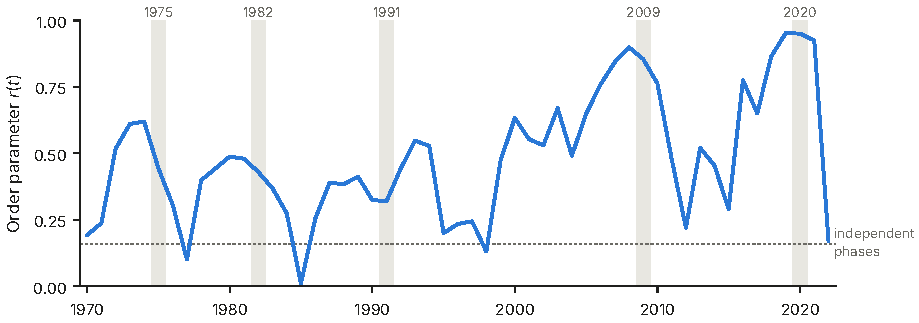
\includegraphics[width=1\linewidth,height=\textheight,keepaspectratio,alt={Figure 1 (F1.3). The Kuramoto order parameter r(t) of the 31 economies, 1970--2022, convention P. Grey bands: the five global recessions. Dotted line: the mean of r under independent random phases.}]{figures/F1-03_order_parameter_s31.pdf}
\caption{\textbf{Figure 1 (F1.3).} The Kuramoto order parameter \(r(t)\) of the 31 economies, 1970--2022, convention P. Grey bands:
the five global recessions. Dotted line: the mean of \(r\) under independent random phases.}
\end{figure}

\subsection{4.1 Synchronization and swing size move together}\label{synchronization-and-swing-size-move-together}

When the economies' cycles are more aligned, they are also larger. After removing slow trends, the correlation between
\(r(t)\) and the mean swing size \(\bar A(t)\) is +0.646 over 1970--2022 (Figure 2, F4.1).
No circular shift of one series against the other does better (\(p =\) 0.019, the floor), and no
one of 5,000 sets of spectrum-preserving surrogate economies does either (\(p =\) 0.0002, the
floor). The link holds on the 30 (+0.641) and the original 26
(+0.608), without Iran and Saudi Arabia, whose swings are the largest
(+0.625), and under every phase convention, including phases from past data
only (+0.726); its size depends on the convention (§3.6.2). This test uses no
recession dates.

\begin{figure}
\centering
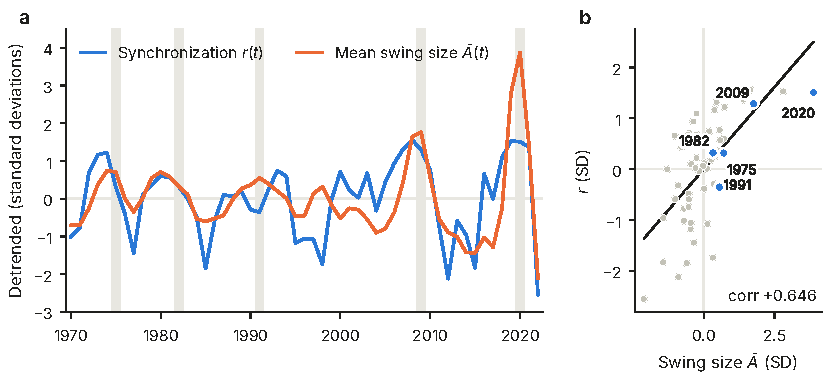
\includegraphics[width=1\linewidth,height=\textheight,keepaspectratio,alt={Figure 2 (F4.1). Synchronization and swing size. (a) r(t) and the mean swing size \textbackslash bar A(t), each minus a Gaussian-smoothed trend (\textbackslash sigma = 8 years) and standardized; grey bands: global recessions. (b) The same 53 years as pairs, recession years in blue, with the least-squares line.}]{figures/F4-01_amplitude_s31.pdf}
\caption{\textbf{Figure 2 (F4.1).} Synchronization and swing size. (a) \(r(t)\) and the mean swing size \(\bar A(t)\), each minus a
Gaussian-smoothed trend (\(\sigma = 8\) years) and standardized; grey bands: global recessions. (b) The same 53 years as
pairs, recession years in blue, with the least-squares line.}
\end{figure}

\subsection{4.2 Recession variance is mostly co-movement}\label{recession-variance-is-mostly-co-movement}

In global recessions the world economy loses diversification: the economies' cycles stop offsetting one another. On
rolling 10-year windows the variance of the GDP-weighted world cycle splits exactly into an own term (each economy's
volatility) and a cross term (co-movement). The cross term supplies
84.3\% of the extra world variance in recession windows
(97.0\% with equal weights; on the 30,
83.3\% and 96.8\%;
Figure 3, F4.4). This is a descriptive magnitude, not a significance claim: the share has no proper null (§3.6.6), and
the cross term dominates world variance in any period because 465 pairs outnumber 31 variances (§3.5.1). What is
specific to recessions is the gap: the cross term's share of world variance is
0.706 in recession windows against
0.620 in normal ones.

The cross term rises for two reasons, and they are of similar size. Raising only the pairwise correlations from their
normal to their recession means supplies 46\% of its rise; raising only
the swing sizes supplies 40\%; their interaction the remaining
14\%. We read this as \textbf{amplification transmitted by alignment}: larger
swings matter for world output because they are aligned, and which of the two parts is larger depends on the sample
(on the original 26, swing size 53\% against correlation
33\%).

The same arithmetic can be written for a single year (Box 1, §5.2). If a common shock reaches each economy according to
where it is in its cycle, the world response has the variance of \(N_{\mathrm{eff}} = 1/r^2\) independent economies:
with the phases spread out the 31 economies behave like 31, with the phases aligned they behave like one. Over
1970--2022, \(N_{\mathrm{eff}} = 1/E[r^2]\) is about 3.5 on average,
2.4 in recession years and
2.1 in the year before, and
1.1 in 2020 (descriptive; Appendix Table A7). The dip is carried by
2009 (1.37) and 2020
(1.11); the earlier recession years are not low
(1975 5.1, 1982 5.4,
1991 9.8). Averaged over the decomposition's windows the variance law
gives the cross term 84.1\% of the extra
recession variance, against the 84.3\% measured:
the loss of diversification is this arithmetic, and it is an accounting of the recession excess, not a cause of it.

\begin{figure}
\centering
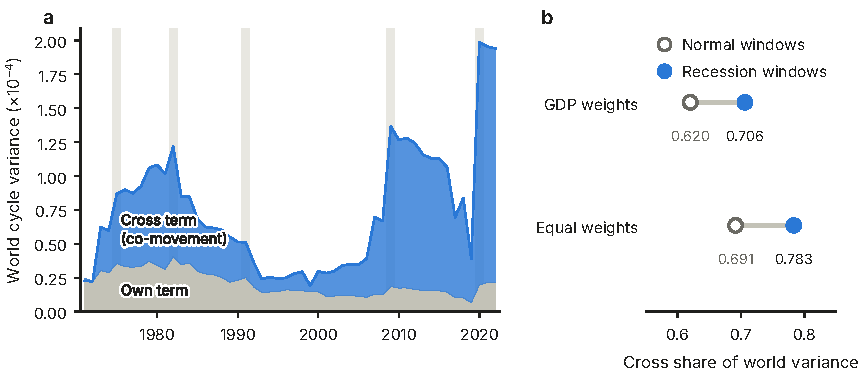
\includegraphics[width=1\linewidth,height=\textheight,keepaspectratio,alt={Figure 3 (F4.4). Loss of diversification. (a) Variance of the GDP-weighted world cycle on 10-year windows, split into the own term (grey) and the cross term (blue); grey bands: windows ending in a recession year. (b) The cross term's share of world variance in normal and recession windows, with GDP and with equal weights. No p-value is shown: the share has no proper null (§3.6.6).}]{figures/F4-04_diversification_s31.pdf}
\caption{\textbf{Figure 3 (F4.4).} Loss of diversification. (a) Variance of the GDP-weighted world cycle on 10-year windows,
split into the own term (grey) and the cross term (blue); grey bands: windows ending in a recession year. (b) The cross
term's share of world variance in normal and recession windows, with GDP and with equal weights. No p-value is shown:
the share has no proper null (§3.6.6).}
\end{figure}

\subsection{4.3 The network has tightened}\label{the-network-has-tightened}

The correlation network of the 31 business cycles has tightened over five decades. The mean edge length of its minimum
spanning tree fell from 0.687 in 1979--89 to 0.424
in 2013--22, a factor of 1.6× (Figure 4, F5.1; 1.6× on the 30 and
1.8× on the original 26). This is a description of a trend, not a test. The network does not contract
in the years before recessions (\(\tau =\) −0.157, \(p =\) 0.206; §3.5.5), and the
economies move too nearly together for a leader to be identified: the spread of their phase leads is
0.546 years, below every one of 5,000 surrogates (\(p =\) 0.0002,
the floor; §3.5.6).

\begin{figure}
\centering
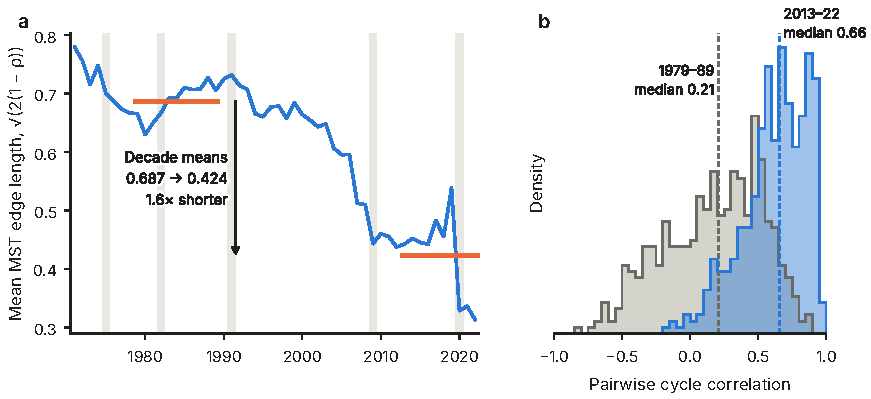
\includegraphics[width=1\linewidth,height=\textheight,keepaspectratio,alt={Figure 4 (F5.1). The network has tightened. (a) Mean edge length of the minimum spanning tree of the 31 business cycles on 10-year windows, with the decade means for 1979--89 and 2013--22 (orange). (b) The 465 pairwise cycle correlations, averaged over the windows ending in each decade; dashed lines: medians.}]{figures/F5-01_mst_s31.pdf}
\caption{\textbf{Figure 4 (F5.1).} The network has tightened. (a) Mean edge length of the minimum spanning tree of the 31 business
cycles on 10-year windows, with the decade means for 1979--89 and 2013--22 (orange). (b) The 465 pairwise cycle
correlations, averaged over the windows ending in each decade; dashed lines: medians.}
\end{figure}

\subsection{4.4 Synchronization rises in the year before global recessions}\label{synchronization-rises-in-the-year-before-global-recessions}

With phases built from past data only --- the version that uses no information from after each year --- synchronization
is higher in the year before global recessions: the lead-1 correlation is +0.379
(\(p =\) 0.038 against 53 circular shifts, whose floor is 0.019), \textbf{and it rests on two
events, 2009 and 2020 (\(n \approx 2\))}: without either the two-sided lead is not significant (\(p =\)
0.226 and 0.283), and without both it is
gone (−0.02). With China left out the past-only lead-1 is
+0.357 (\(p =\) 0.057). With the
usual two-sided phases the lead-1 correlation is +0.231, at the floor of the circular-shift
null (\(p =\) 0.019) and \(p =\) 0.033 against
surrogates with ends (§3.4.4); it survives the removal of any one of the 31 economies (\(p \le\)
0.038; Appendix Table A3) and the edge-robust convention (\(p =\)
0.019), but not convention N (\(p =\) 0.057), and it does
not pass a correction for testing five lags, which with 53 shifts a single lag cannot do (§3.6.4). We lead with the
past-only value because the two-sided arc is inflated by how recessions are dated (Limitations). On the 30 the
past-only lead-1 is +0.369 (\(p =\) 0.038) and on the 26
+0.374 (\(p =\) 0.038).

The rest of the arc is not claimed (Figure 5, F2.5). The two-year lead (lead-2 +0.235,
\(p =\) 0.038) does not survive past-only phases (−0.044,
\(p =\) 0.585). The crisis year is not significant with two-sided phases
(\(p =\) 0.189); with past-only phases it is at the floor
(+0.417, \(p =\) 0.019), which was not a
pre-registered claim and is reported, not interpreted. The fall two years after recessions
(−0.258, \(p =\) 0.057) is in the Limitations. This is a property of the
tightly coupled modern economy, observed twice; it is not a fifty-year regularity and not a forecast.

\begin{figure}
\centering
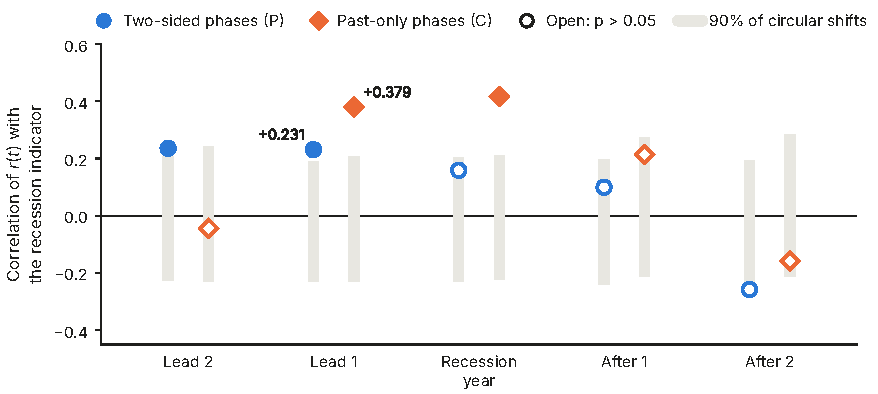
\includegraphics[width=1\linewidth,height=\textheight,keepaspectratio,alt={Figure 5 (F2.5). The tested arc. Correlation of r(t) with the recession indicator at each lag, with two-sided phases (P, circles) and phases from past data only (C, diamonds). Filled: one-sided p \textbackslash le 0.05 against 53 circular shifts (floor 0.019); grey bars: the range of 90\% of the shifted correlations.}]{figures/F2-05_arc_tested_s31.pdf}
\caption{\textbf{Figure 5 (F2.5).} The tested arc. Correlation of \(r(t)\) with the recession indicator at each lag, with two-sided
phases (P, circles) and phases from past data only (C, diamonds). Filled: one-sided \(p \le 0.05\) against 53 circular
shifts (floor 0.019); grey bars: the range of 90\% of the shifted correlations.}
\end{figure}

\subsection{4.5 No critical slowing down}\label{no-critical-slowing-down}

Before recessions the variance of synchronization rises (\(\tau =\) +0.438, \(p =\)
0.031 against 5,000 surrogates; \(p =\) 0.029 against
surrogates with ends) while its lag-1 autocorrelation does not (\(\tau =\) −0.152, \(p =\)
0.789), and the recovery rate does not fall after recessions (\(p =\)
0.502; Figure 6, F6.1). Critical slowing down --- the signature of a system approaching
a bifurcation --- raises variance and autocorrelation together, because both come from a slower return to equilibrium.
A rise in variance alone is not that signature. \emph{As an interpretation, not a test:} it is what noise-induced tipping
would show, where larger disturbances push the system across a threshold while its restoring forces stay the same
(Ashwin et al.~2012). The variance rise, like the lead, rests on 2009 and 2020 (before them alone
+0.857, \(p =\)
0.003; before 1982 and 1991,
+0.018, \(p =\)
0.513; Appendix Table A8), and it is significant under
conventions P and E but not W or N (§3.5.7).

\begin{figure}
\centering
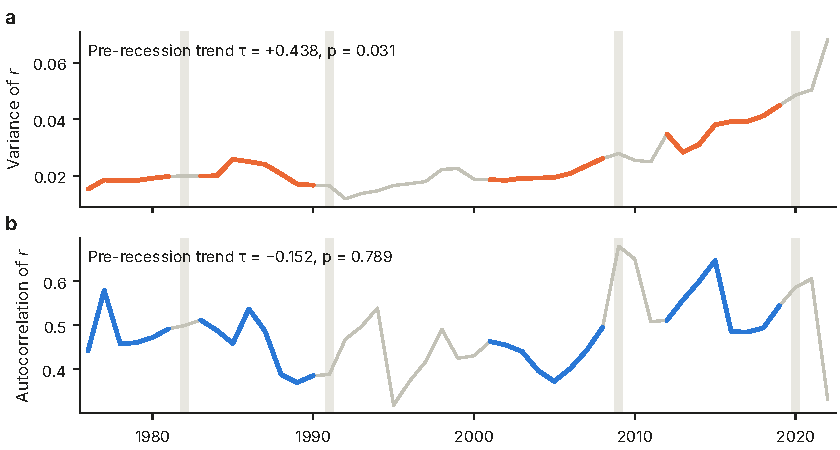
\includegraphics[width=1\linewidth,height=\textheight,keepaspectratio,alt={Figure 6 (F6.1). No critical slowing down. Variance (a) and lag-1 autocorrelation (b) of the fluctuations of r(t) on trailing 15-year windows. In colour: the eight years before each recession, over which the trend is tested; grey bands: recession years.}]{figures/F6-01_early_warning_s31.pdf}
\caption{\textbf{Figure 6 (F6.1).} No critical slowing down. Variance (a) and lag-1 autocorrelation (b) of the fluctuations of
\(r(t)\) on trailing 15-year windows. In colour: the eight years before each recession, over which the trend is tested;
grey bands: recession years.}
\end{figure}

\section{5 Discussion}\label{discussion}

\subsection{5.1 What the transition is, and what it is not}\label{what-the-transition-is-and-what-it-is-not}

We first asked whether global recessions arrive the way a system approaches a bifurcation, with recovery slowing as a
threshold nears. They do not: before recessions the autocorrelation of synchronization does not rise, and after them
the recovery rate does not fall (§4.5). That ``what it isn't'' led to the account the paper proposes: loss of
diversification. In recessions the economies' cycles stop offsetting one another, and co-movement supplies most of the
extra world variance (§4.2). Because co-movement and larger swings contribute about equally, we read the recession
excess as amplification transmitted by alignment: shocks that would have cancelled across economies are passed along
instead. The rise in the variance of synchronization before recessions, without a rise in its autocorrelation, fits
the same reading --- when shocks stop cancelling, synchronization swings more widely without recovering more slowly ---
and in the taxonomy of Ashwin et al.~(2012) it is what noise-induced rather than bifurcation-induced tipping would
show. This is a reading of the data, not a separate test, and it rests on 2009 and 2020.

\subsection{5.2 Box 1: loss of diversification as arithmetic}\label{box-1-loss-of-diversification-as-arithmetic}

\begin{tcolorbox}[enhanced,breakable,colback=boxgrey,colframe=boxgrey,boxrule=0pt,arc=0pt,left=10pt,right=10pt,top=8pt,bottom=8pt,before upper={\setlength{\parskip}{5pt}}]
\textbf{Box 1 \textbar{} Why aligned cycles stop diversifying}

Let economy \(i\)'s cycle have phase \(\theta_i\) and swing size \(A_i\), and let a shock reach every economy according to
where it is in its cycle: economy \(i\) responds with \(q_i = \sigma A_i\, u\cdot v_i\), where \(v_i = (\cos\theta_i,
\sin\theta_i)\) and \(u\) is a unit direction drawn at random. The same disturbance pushes an economy near its peak down
and one near its trough up, so economies at opposite points of their cycles cancel in the world average. If only a
share \(\rho\) of the shock is common and the rest is independent across economies (each with variance
\(\sigma^2A_i^2/2\)), the variance of the world-average response \(\bar q\), given the phases, is
\[\mathrm{Var}(\bar q) = \frac{\sigma^2}{2}\Big[\rho\,|Z_A|^2 + (1-\rho)\,\frac{\overline{A^2}}{N}\Big], \qquad Z_A = \frac{1}{N}\sum_i A_i e^{\mathrm{i}\theta_i}.\]
The first term is the common shock, the second the independent part. Because \(|Z_A| = \bar A\, R_A\), with
\(R_A = |\sum_i A_i e^{\mathrm{i}\theta_i}| / \sum_i A_i\) the alignment weighted by swing size, the common term is
the square of an exact identity: world swing equals mean swing size times alignment. With equal swing sizes and a
fully common shock, \(\mathrm{Var}(\bar q) = \sigma^2 r^2/2\), against \(\sigma^2/(2N)\) if the responses were
independent. The world then varies like
\[N_{\mathrm{eff}} = 1/r^2\]
independent economies: the number that would give the same world variance if they did not move together. With a
common share \(\rho\), \(N_{\mathrm{eff}} = 1/(\rho r^2 + (1-\rho)/N)\). Alignment matters only for the common part of
shocks. The independent part is the averaging-out of Lucas (1977), which fails when a few units are large (Gabaix
2011) or central in the input--output network (Acemoglu et al.~2012); here it fails for a third reason: the
economies' cycles line up.

On the 31 economies \(N_{\mathrm{eff}} = 1/E[r^2]\) is about 3.5 over
1970--2022, 2.4 in recession years and
2.1 the year before
(1.1 in 2020); 2009 and 2020 pull these down, and the earlier
recessions are not low. Averaged over the 10-year windows of §4.2, the law gives the cross term
84.1\% of the extra world variance in
recession windows, against 84.3\% measured.

\textbf{It is arithmetic, not a mechanism.} Any year in which cycles happen to line up has a larger world swing, coupled
or not, and recessions dated from world output are such years even in simulated worlds with no coupling (§5.4).

\emph{Interpretation, not a test:} in the taxonomy of Ashwin et al.~(2012), a transition caused by larger disturbances
while the restoring forces stay the same is noise-induced tipping, which does not show critical slowing down --- and the
autocorrelation of synchronization does not rise before recessions, nor does recovery slow after them (§4.5).
\end{tcolorbox}

The law is exact for the stated shock, which we check against simulation (the code is in the repository); its link to
the decomposition is exact year by year (with equal weights and swing sizes, the cross share is \(1 - N_{\mathrm{eff}}/N\))
and close, not exact, over the decomposition's windows. With GDP weights the independent term becomes
\((1-\rho)\sum_i w_i^2A_i^2/2\), a Herfindahl-type concentration --- Gabaix's granular channel --- and the common term
\(\rho\,|\sum_i w_iA_ie^{\mathrm{i}\theta_i}|^2/2\) is the alignment channel. The two are complements, not rivals.

\subsection{5.3 Diversification-type tipping}\label{diversification-type-tipping}

We call a transition of this kind diversification-type tipping: a transition caused by losing the cancellation between
economies rather than by slowing recovery. It differs from bifurcation-induced tipping, which shows the slowing-down
signature we do not find. In finance, ``diversification'' and systemic risk usually describe a different mechanism ---
institutions that each diversify become alike and more connected, so diversification itself can spread distress
(Burkholz, Garas and Schweitzer 2016) --- and our sense is narrower: cycles that stop offsetting one another. This paper
does not show that loss of diversification has a threshold, a level of coupling beyond which cancellation fails
abruptly rather than gradually.

\subsection{5.4 The mechanism check: simulated worlds with known coupling}\label{the-mechanism-check-simulated-worlds-with-known-coupling}

Two simulation studies, each pre-registered before it was run, ask what the tests can and cannot show.

\textbf{G1: worlds with known coupling.} We simulated 31 economies as phase oscillators (Kuramoto) and as phase-and-size
oscillators (Stuart--Landau) on the real trade network, calibrated to the real cycles, and ran every test of this paper
on 1,000 worlds per setting. With no coupling the tests reject at about their stated rates (Table 1, §3.4.3). Two
findings bear on the claims. First, when recessions are dated from each simulated world's own output, as global
recessions are, the two-sided crisis-year and lead-1 arcs reject in 8.2\%--8.9\%
and 8.5\%--8.6\% of uncoupled worlds, about twice the correct
rate, while the past-only lead-1 does not (2.3\%--2.9\%): this is
why the lead claim rests on the past-only version. Second, no G1 world produced the past-only lead: with own-dated
recessions it rejected in 1.7\% of trade-coupled,
2.9\% of uncoupled and 2.5\% of
commonly forced Kuramoto worlds, never above chance.

\textbf{G1b: a synchrony-driven escape layer.} We then added the mechanism Box 1 suggests to the same Kuramoto worlds: a
recession is an escape of a world-level state from a stable well, \(dx = (\mu + x - x^3)\,dt + \sigma\,r(t)\,dW\), so that
shocks grow with the worlds' true synchrony. \(\sigma\) was set so that worlds have five recession years in 53 on
average, using only their number, never their timing; each escape resets the state and starts a two-year refractory
period. Before running we fixed what ``reproduces the lead'' means: (a) the past-only lead-1 rejects more often than
chance (the lower bound of its 95\% interval above 3.8\%); (b) more often than the same layer with constant noise and
with synchrony shuffled in time (both paired differences' intervals above zero); and (c) at least 20\% of worlds reach
the real \(p =\) 0.038. Some lead is expected by construction, since the layer makes
recessions likelier when synchrony is high; the question is how much survives annual sampling, 53 points, five events
and past-only phases.

The verdict, exactly as pre-registered, is \textbf{partly} (Appendix Table A11). In
trade-coupled worlds the past-only lead-1 rejects in 6.3\% of worlds (95\%
interval 5.0\%--8.0\%), above chance (a) and above
both controls (b: 3.5 percentage points more than with constant noise,
3.4 percentage points more than with shuffled synchrony). But only
6.3\% of worlds reach the real \(p\), against the 20\% required (c fails),
and 1.3\% reach the real correlation of
+0.379. Without trade coupling the layer leaves no past-only lead
(4.0\% with no coupling, 3.2\% with common
forcing only). Of eight pre-registered sensitivities on the trade-coupled worlds, 6 give the
same verdict and 2 do not reproduce the lead (one state per economy; refractory 4 years); none
reaches (c).

What this says, and no more: a synchrony-driven escape mechanism on coupled economies can leave a past-only lead that
our pipeline detects, and coupling is needed for it, but a lead as large as the real one is rare under it. Either the
real lead is an unusual draw --- which, resting on two events, it may well be --- or the real mechanism is stronger than,
or different from, the one simulated; the simulated recessions, for instance, do not feed back on the cycles they are
measured from. We claim no mechanism from this check.

\subsection{5.5 Where this sits}\label{where-this-sits}

The world business-cycle factor of Kose, Otrok and Whiteman (2003) measures how much economies move together; we ask
when they do, and whether togetherness itself is the danger. Treating national cycles as coupled oscillators follows
Selover and Jensen (1999), who described mode-locking of business cycles, and Ikeda, Aoyama and Yoshikawa (2013), who
fitted Kuramoto-type couplings between six economies' quarterly cycles; Pangallo (2025) shows that trade can
synchronize endogenous cycles across 24 countries. Morikawa, Morikawa and Nakamichi (2026) use the same Hilbert and
Kuramoto toolkit for a different question, the 1/f spectra of economic series. None of these relates synchronization to
the timing of global recessions or to the loss of diversification. We do not forecast: two-sided filters cannot support
a forecast, and the past-only lead rests on two events.

\section{6 Limitations}\label{limitations}

\textbf{Two events carry the lead and the variance rise.} The pre-recession rise rests on 2009 and 2020 (\(n \approx 2\)):
without either the two-sided lead-1 is not significant (\(p =\) 0.226 and
0.283), the split sample 1970--1995 shows none (lead-1
+0.24, \(p =\) 0.154), and
the variance rise of §4.5 has the same dependence. Both are properties of the tightly coupled modern economy observed
twice, not regularities, and with five events in 53 years no test here has more than five degrees of freedom.

\textbf{What multiplicity correction can show.} No lag survives a correction for testing five lags. With 53 circular shifts
the smallest \(p\) the test can return is 0.019, so a single lag can never pass Bonferroni and passes Benjamini--Hochberg
only alongside another lag at the floor, which happened on the original 26 but not on the 30 or the 31 (Appendix
Table A5). The pre-crisis rise therefore rests on its survival under past-only phases and leave-one-economy-out, not on
corrected significance.

\textbf{How global recessions are dated.} Global recessions are dated from world output, and the economies whose
synchronization we measure make up most of it. The years in which world output falls most are years in which many
cycles happen to be falling together, so dating recessions this way builds some synchronization into them even when
economies are not coupled at all. In simulated worlds with no coupling, recession years dated the same way from each
world's own output make the two-sided arc reject at the crisis year in
8.2\%--8.9\% and at lead-1 in
8.5\%--8.6\% of worlds, about twice the correct 3.8\% (§3.4.3).
Phases built from past data only are free of this (2.3\%--2.9\%).
The lead claim therefore rests on the past-only lead-1 (+0.379,
\(p =\) 0.038), not on the two-sided one.

\textbf{What the cross-term test shows.} The surrogate test of the cross term (§3.6.6) asks whether the cross term's share of
world variance in recession windows exceeds what independent economies would give. In simulated worlds it rejects in
nearly every coupled world whatever dates are used --- 97.1\%--99.3\%
of trade-coupled worlds with the real recession dates, which have nothing to do with those worlds --- and in about 5\% of
uncoupled ones. It detects co-movement in general, not co-movement at recessions. The recession-specific claim --- that
co-movement supplies more of world variance in recessions than in normal years --- rests on the gap between recession
and normal windows (cross share 0.706 against
0.620, GDP-weighted), which is descriptive.

\textbf{The end of the sample.} 2020 sits two years from the last observation, and both the forward--backward filter and the
Hilbert transform are least reliable there. Without 2020 the two-sided lead-1 is +0.11
(\(p =\) 0.283). Surrogates with ends (§3.4.4) move the two-sided lead-1 from
0.019 to 0.033
and leave the claimed results on the same side of 0.05, but the most recent event remains the least well measured;
data for 2023--2025 are the cleanest fix.

\textbf{The fall after recessions.} Synchronization falls in the two years after a global recession (lag \(-2\):
−0.258 on the 31, \(p =\) 0.057; −0.236,
\(p =\) 0.057 on the 30; −0.277, \(p =\) 0.019 on the
original 26), but this half of the arc does not hold up. It is not significant on the 31 or the 30; it disappears with
the 3--10 year band and with growth rates (§3.6.1--3.6.2); it is significant under none of the alternative phase
conventions, including phases from past data only; and without 2020 it is −0.18
(\(p =\) 0.151). On the 31 it sits on the threshold: leaving out any of
20 of the 31 economies, or computing Russia's phases from 1992, takes it below 0.05. It
also sits where the filters are least reliable: the lag \(-2\) test for 2020 uses \(r(2022)\), the last observation.
Against surrogates with ends it is \(p =\) 0.039 on the 31 and
0.054 on the 30; that null still rejects lag \(-2\) slightly too
often in simulated coupled worlds (6.5\%), and most of the move is the finer
resolution of 5,000 surrogates against 53 shifts. We report it and do not claim it.

\textbf{Phase conventions.} The arc depends on where the Hilbert transform is applied (Table 2). Lead-1 is significant under
P, W, E and C but not N (\(p =\) 0.057), and on the 30 not under W
(\(p =\) 0.057); the variance rise is significant under P and E but not W or N. The
synchronization--swing-size link holds under all five, with sizes from +0.547 to
+0.726. We chose P before running anything on the added economies, on the ground
that its run-in protects 1970 from edge transients, not because it gives larger values.

\textbf{The dropped rate lead.} With two-sided phases short-term interest rates are most synchronized two years before
global recessions (+0.273, \(p =\) 0.019,
19 economies with continuous rates), but with phases from past data only the rise is gone
(+0.165, \(p =\) 0.151). We make no claim
that rates or investment signal recessions in advance; the channel ordering is description only (Appendix Table A10).

\textbf{The alignment share is sample-sensitive.} Splitting the recession excess in world swing (the identity of Box 1)
into alignment and swing size gives an alignment share of 28\% on the 31,
19\% on the 30, 33\% on the 30 without Iran
and 39\% on the original 26. The swing-size part is significant on every sample
(\(p =\) 0.0002, the floor, also against surrogates with ends); the alignment part on none
(\(p =\) 0.239 on the 31). The share depends on which economies are in the sample, and we draw no
conclusion from it.

\textbf{The mechanism check is narrow.} G1b tested one mechanism in one family of simulated worlds (Kuramoto oscillators on
the real 1970--2022 trade network), with recessions that do not feed back on the cycles and a calibration that fixes only how
often recessions happen. Its \emph{partly} verdict says that this mechanism can leave a detectable past-only lead, not that
it produces the real one.

\textbf{Data.} Annual data give 53 points; Maddison's PPP series for Russia before 1991 are back-cast Soviet-era estimates
(every test is repeated with Russia's phases from 1992); Maddison's 1991--2011 growth for Norway, Switzerland and South
Africa runs above national accounts (replacing it changes no conclusion; §3.6.8). The five recession dates are those of
Kose, Sugawara and Terrones (2020) for 1975--2009 and of the World Bank (2020) for 2020, under the same definition.

\section{7 Future work}\label{future-work}

Paper 1 is closed to new tests. What follows is the programme for a second paper, which has not been started.

\textbf{A graph neural network of coupled economies (stages G2--G4).} A first stage built yearly graphs of the 31 economies
with pinned trade, bank-lending and oil links and a world node (G0), and a simulator of coupled economies with known
coupling run through this paper's pipeline (G1, used in §5.4). The next stages are: G2, a recoverability benchmark that
asks which couplings 53 annual points can reveal at all, and by which method; G3, a model of the real network, trained
only after G2 and checked against a twin with no network, shuffled edges, leave-one-recession-out validation, past-only
phases and classical baselines (a trade-weighted global VAR, a Kuramoto regression, a network autoregression); and G4,
explanations of what the model learned, counted only after the same explanation method recovers known links in the
simulator. The aim is to understand which links carry synchronization, not to forecast recessions.

\textbf{Channel experiments.} The channels inside each economy (interest rates, investment, trade, budgets) synchronize at
different times around recessions with two-sided phases, but no channel lead survives past-only phases. Testing the
ordering properly needs the channel data to be extended and the past-only design to be fixed in advance for each
channel.

\textbf{The remaining DTT modules.} The diversification-type tipping report (Sid, 13 October 2026) has modules this paper
does not use: cascades between economies, asymmetric restoring forces and hysteresis. Each needs its own
pre-registration and a check in the simulator, where the coupling can be raised step by step to test whether loss of
diversification has a threshold. Rate-induced tipping, where the speed of a change rather than its size causes the
transition, is a further hypothesis for that work.

\textbf{Data for 2023--2025.} The most recent recession sits two years from the end of the sample, where the filters are least
reliable. Extending the series by three years, when Maddison's next release covers them, is the cleanest test of the
2020 result and of the fall after recessions.

\textbf{A quarterly track.} Quarterly national accounts would give four times as many points but start around 1981 and lose
the 1975 recession; a quarterly version is a test of whether the annual results survive finer timing, not a
replacement.

\textbf{Banking-crisis dating.} The dates of systemic banking crises (the Jordà--Schularick--Taylor database), tried early in
this project, were not re-verified on pinned data; no claim here depends on them.

\section{AI-assistance disclosure}\label{ai-assistance-disclosure}

This paper was written with substantial help from AI tools, and we say so plainly. Claude (Anthropic) was used for
analysis, code and drafting: it wrote and ran most of the code in the repository that accompanies the paper (the data
build, the pipeline, the tests, the simulations and the figures), drafted text that the author revised, and checked
references. The report on diversification-type tipping that Box 1 draws on (Sid Shinde, 13 October 2026) was drafted
with an OpenAI tool; its equations were re-implemented and checked independently before any of them was used here.
Every number in the paper is produced by code in the repository from pinned data, and every hypothesis, test direction
and sample was written down and committed before the tests were run. The research questions, the choices among
alternatives and the claims are the author's, and the author is responsible for any errors.

\section{References}\label{references}

Acemoglu, D., Carvalho, V. M., Ozdaglar, A. and Tahbaz-Salehi, A. (2012). The network origins of aggregate
fluctuations. \emph{Econometrica} 80(5), 1977--2016. doi:10.3982/ECTA9623.

Ashwin, P., Wieczorek, S., Vitolo, R. and Cox, P. (2012). Tipping points in open systems: bifurcation, noise-induced
and rate-dependent examples in the climate system. \emph{Philosophical Transactions of the Royal Society A} 370(1962),
1166--1184. doi:10.1098/rsta.2011.0306.

Bolt, J. and van Zanden, J. L. (2024). Maddison-style estimates of the evolution of the world economy: a new 2023
update. \emph{Journal of Economic Surveys} 39(2), 631--671 (2025 print issue). doi:10.1111/joes.12618.

Burkholz, R., Garas, A. and Schweitzer, F. (2016). How damage diversification can reduce systemic risk. arXiv
1503.00925. {[}Journal version reported as \emph{Physical Review E} 93, 042313: \textbf{unverified}.{]}

Gabaix, X. (2011). The granular origins of aggregate fluctuations. \emph{Econometrica} 79(3), 733--772.
doi:10.3982/ECTA8769.

Ikeda, Y., Aoyama, H. and Yoshikawa, H. (2013). Synchronization and the coupled oscillator model in international
business cycles. RIETI Discussion Paper 13-E-089.

Kose, M. A., Otrok, C. and Whiteman, C. H. (2003). International business cycles: world, region, and country-specific
factors. \emph{American Economic Review} 93(4), 1216--1239. doi:10.1257/000282803769206278.

Kose, M. A., Sugawara, N. and Terrones, M. E. (2020). Global recessions. World Bank Policy Research Working Paper 9172.
doi:10.1596/1813-9450-9172.

Kose, M. A. and Terrones, M. E. (2015). \emph{Collapse and Revival: Understanding Global Recessions and Recoveries}.
Washington, DC: International Monetary Fund. doi:10.5089/9781484370414.071.

Kuramoto, Y. (1984). \emph{Chemical Oscillations, Waves, and Turbulence}. Springer Series in Synergetics 19. Berlin:
Springer. doi:10.1007/978-3-642-69689-3.

Lucas, R. E., Jr.~(1977). Understanding business cycles. \emph{Carnegie-Rochester Conference Series on Public Policy} 5,
7--29. {[}The attribution of the averaging-out argument to this paper is verified through the papers that cite it; the
original text was not read.{]}

Mantegna, R. N. (1999). Hierarchical structure in financial markets. \emph{European Physical Journal B} 11, 193--197.
doi:10.1007/s100510050929.

Morikawa, M., Morikawa, Y. and Nakamichi, A. (2026). Pink noise in economic time series from synchronization and
amplitude demodulation. arXiv 2605.17490.

Pangallo, M. (2025). Synchronization of endogenous business cycles. \emph{Journal of Economic Behavior \& Organization} 229,
106827.

Pikovsky, A., Rosenblum, M. and Kurths, J. (2001). \emph{Synchronization: A Universal Concept in Nonlinear Sciences}.
Cambridge: Cambridge University Press.

Scheffer, M., Bascompte, J., Brock, W. A., Brovkin, V., Carpenter, S. R., Dakos, V., Held, H., van Nes, E. H.,
Rietkerk, M. and Sugihara, G. (2009). Early-warning signals for critical transitions. \emph{Nature} 461, 53--59.
doi:10.1038/nature08227.

Selover, D. D. and Jensen, R. V. (1999). `Mode-locking' and international business cycle transmission. \emph{Journal of
Economic Dynamics and Control} 23(4), 591--618.

Shinde, S. (2026). DTT: diversification-type tipping --- unified mathematical simulation report. Unpublished report,
13 October 2026 (in the repository as a frozen record).

Theiler, J., Eubank, S., Longtin, A., Galdrikian, B. and Farmer, J. D. (1992). Testing for nonlinearity in time series:
the method of surrogate data. \emph{Physica D} 58, 77--94. doi:10.1016/0167-2789(92)90102-S.

World Bank (2020). \emph{Global Economic Prospects, June 2020}. Washington, DC: World Bank. {[}That it dates 2020 as a global
recession under the Kose--Sugawara--Terrones definition is from its Box 1.1 as summarized in secondary sources; the box
itself was not read: \textbf{partly unverified}.{]}

\section{Appendix}\label{appendix}

All values are convention P unless a row says otherwise; one-sided \(p\) in brackets. Circular-shift \(p\)-values have a
floor of \(1/53 = 0.019\) (for the split samples of 26 and 27 years, 0.038 and 0.037); surrogate \(p\)-values with 5,000 draws have
a floor of 0.0002, with 2,000 draws 0.0005.

\subsection{Table A1. Key results by sample}\label{table-a1.-key-results-by-sample}

The original 26 economies, the 30 (without Russia), the 31, the 31 without each added economy, with Russia's phases from
1992 only and without Iran and Saudi Arabia together. ``---'': not run (the variant without Iran and Saudi Arabia was
pre-registered for the swing-size tests only, the one with Russia from 1992 for the circular-shift tests only).

{\def\LTcaptype{none} % do not increment counter
\begin{longtable}[]{@{}
  >{\raggedright\arraybackslash}p{(\linewidth - 20\tabcolsep) * \real{0.2857}}
  >{\raggedright\arraybackslash}p{(\linewidth - 20\tabcolsep) * \real{0.0714}}
  >{\raggedright\arraybackslash}p{(\linewidth - 20\tabcolsep) * \real{0.0714}}
  >{\raggedright\arraybackslash}p{(\linewidth - 20\tabcolsep) * \real{0.0714}}
  >{\raggedright\arraybackslash}p{(\linewidth - 20\tabcolsep) * \real{0.0714}}
  >{\raggedright\arraybackslash}p{(\linewidth - 20\tabcolsep) * \real{0.0714}}
  >{\raggedright\arraybackslash}p{(\linewidth - 20\tabcolsep) * \real{0.0714}}
  >{\raggedright\arraybackslash}p{(\linewidth - 20\tabcolsep) * \real{0.0714}}
  >{\raggedright\arraybackslash}p{(\linewidth - 20\tabcolsep) * \real{0.0714}}
  >{\raggedright\arraybackslash}p{(\linewidth - 20\tabcolsep) * \real{0.0714}}
  >{\raggedright\arraybackslash}p{(\linewidth - 20\tabcolsep) * \real{0.0714}}@{}}
\toprule\noalign{}
\begin{minipage}[b]{\linewidth}\raggedright
Quantity
\end{minipage} & \begin{minipage}[b]{\linewidth}\raggedright
S26
\end{minipage} & \begin{minipage}[b]{\linewidth}\raggedright
S30
\end{minipage} & \begin{minipage}[b]{\linewidth}\raggedright
S31
\end{minipage} & \begin{minipage}[b]{\linewidth}\raggedright
S31 without China
\end{minipage} & \begin{minipage}[b]{\linewidth}\raggedright
without Brazil
\end{minipage} & \begin{minipage}[b]{\linewidth}\raggedright
without Saudi Arabia
\end{minipage} & \begin{minipage}[b]{\linewidth}\raggedright
without Iran
\end{minipage} & \begin{minipage}[b]{\linewidth}\raggedright
without Russia (= S30)
\end{minipage} & \begin{minipage}[b]{\linewidth}\raggedright
Russia from 1992
\end{minipage} & \begin{minipage}[b]{\linewidth}\raggedright
without Iran and Saudi Arabia
\end{minipage} \\
\midrule\noalign{}
\endhead
\bottomrule\noalign{}
\endlastfoot
Arc, lead-2 & +0.230 (0.038) & +0.226 (0.038) & +0.235 (0.038) & +0.226 (0.057) & +0.225 (0.038) & +0.252 (0.019) & +0.244 (0.038) & +0.226 (0.038) & +0.229 (0.038) & --- \\
Arc, lead-1 & +0.216 (0.019) & +0.217 (0.019) & +0.231 (0.019) & +0.231 (0.019) & +0.224 (0.019) & +0.229 (0.038) & +0.241 (0.019) & +0.217 (0.019) & +0.224 (0.019) & --- \\
Lead-1, past-only phases & +0.374 (0.038) & +0.369 (0.038) & +0.379 (0.038) & +0.357 (0.057) & +0.391 (0.038) & +0.403 (0.038) & +0.373 (0.038) & +0.369 (0.038) & --- & --- \\
Arc, after-2 (lower tail) & −0.277 (0.019) & −0.236 (0.057) & −0.258 (0.057) & −0.262 (0.038) & −0.274 (0.019) & −0.260 (0.038) & −0.274 (0.019) & −0.236 (0.057) & −0.254 (0.038) & --- \\
r with swing size, detrended & +0.608 (0.019; surr. 0.0002) & +0.641 (0.019; surr. 0.0002) & +0.646 (0.019; surr. 0.0002) & +0.656 (0.019; surr. 0.0002) & +0.628 (0.019; surr. 0.0002) & +0.625 (0.019; surr. 0.0002) & +0.650 (0.019; surr. 0.0002) & +0.641 (0.019; surr. 0.0002) & +0.655 (0.019) & +0.625 (0.019; surr. 0.0002) \\
Cross share of the recession excess, GDP weights & 80.2\% & 83.3\% & 84.3\% & 83.1\% & 83.4\% & 83.8\% & 84.0\% & 83.3\% & --- & 83.5\% \\
Same, equal weights & 96.5\% & 96.8\% & 97.0\% & 96.9\% & 96.8\% & 97.3\% & 96.7\% & 96.8\% & --- & 97.0\% \\
Cross-term rise: correlation / swing size / interaction & 33 / 53 / 14\% & 44 / 41 / 15\% & 46 / 40 / 14\% & 41 / 45 / 14\% & 45 / 42 / 14\% & 45 / 41 / 14\% & 44 / 42 / 14\% & 44 / 41 / 15\% & --- & 43 / 43 / 14\% \\
Alignment share of the swing excess (p) & 39.3\% (0.103) & 18.9\% (0.356) & 28.5\% (0.239) & 32.6\% (0.179) & 24.7\% (0.276) & 28.6\% (0.242) & 38.3\% (0.119) & 18.9\% (0.356) & --- & 41.4\% (0.095) \\
MST decade means, 1979--89 vs 2013--22 & 0.677 vs 0.379 (1.79×) & 0.680 vs 0.421 (1.62×) & 0.687 vs 0.424 (1.62×) & 0.682 vs 0.418 (1.63×) & 0.694 vs 0.414 (1.67×) & 0.685 vs 0.416 (1.65×) & 0.684 vs 0.412 (1.66×) & 0.680 vs 0.421 (1.62×) & --- & --- \\
Phase-lead spread (lower-tail p) & 0.445 yr (0.0002) & 0.535 yr (0.0004) & 0.546 yr (0.0002) & 0.535 yr (0.0006) & 0.542 yr (0.0004) & 0.545 yr (0.0006) & 0.474 yr (0.0002) & 0.535 yr (0.0004) & --- & --- \\
Autocorrelation trend before recessions & +0.027 (0.456) & −0.098 (0.676) & −0.152 (0.789) & −0.205 (0.839) & −0.098 (0.684) & +0.009 (0.487) & −0.152 (0.764) & −0.098 (0.676) & --- & --- \\
Variance trend before recessions & +0.438 (0.033) & +0.420 (0.037) & +0.438 (0.031) & +0.438 (0.033) & +0.402 (0.045) & +0.438 (0.031) & +0.420 (0.037) & +0.420 (0.037) & --- & --- \\
Recovery-rate change after recessions & +0.078 (0.534) & +0.024 (0.507) & +0.002 (0.502) & −0.022 (0.480) & −0.017 (0.472) & +0.027 (0.498) & +0.068 (0.517) & +0.024 (0.507) & --- & --- \\
Short-rate synchronization, lead-2 {[}economies{]} & +0.266 (0.019) {[}18{]} & +0.273 (0.019) {[}19{]} & +0.273 (0.019) {[}19{]} & +0.273 (0.019) {[}19{]} & +0.266 (0.019) {[}18{]} & +0.273 (0.019) {[}19{]} & +0.273 (0.019) {[}19{]} & +0.273 (0.019) {[}19{]} & --- & --- \\
\end{longtable}
}

\subsection{Table A2. Robustness of the arc}\label{table-a2.-robustness-of-the-arc}

Correlation of \(r(t)\) with the recession indicator at each lag (one-sided \(p\); after-2 tested downward). 2--9 year band
unless stated.

\emph{The 31 economies.}

{\def\LTcaptype{none} % do not increment counter
\begin{longtable}[]{@{}
  >{\raggedright\arraybackslash}p{(\linewidth - 8\tabcolsep) * \real{0.5000}}
  >{\raggedright\arraybackslash}p{(\linewidth - 8\tabcolsep) * \real{0.1250}}
  >{\raggedright\arraybackslash}p{(\linewidth - 8\tabcolsep) * \real{0.1250}}
  >{\raggedright\arraybackslash}p{(\linewidth - 8\tabcolsep) * \real{0.1250}}
  >{\raggedright\arraybackslash}p{(\linewidth - 8\tabcolsep) * \real{0.1250}}@{}}
\toprule\noalign{}
\begin{minipage}[b]{\linewidth}\raggedright
Check
\end{minipage} & \begin{minipage}[b]{\linewidth}\raggedright
Lead-2
\end{minipage} & \begin{minipage}[b]{\linewidth}\raggedright
Lead-1
\end{minipage} & \begin{minipage}[b]{\linewidth}\raggedright
Crisis year
\end{minipage} & \begin{minipage}[b]{\linewidth}\raggedright
After-2 (lower tail)
\end{minipage} \\
\midrule\noalign{}
\endhead
\bottomrule\noalign{}
\endlastfoot
Baseline & +0.24 (0.038) & +0.23 (0.019) & +0.16 (0.189) & −0.26 (0.057) \\
Band 2--8 years & +0.23 (0.057) & +0.19 (0.094) & +0.12 (0.226) & −0.27 (0.019) \\
Band 3--10 years & +0.26 (0.038) & +0.25 (0.019) & +0.16 (0.132) & +0.00 (0.509) \\
HP filter, λ = 100 & +0.27 (0.038) & +0.29 (0.019) & +0.14 (0.113) & −0.18 (0.094) \\
Growth rates instead of band-pass & +0.25 (0.057) & +0.34 (0.038) & +0.15 (0.132) & +0.04 (0.679) \\
1970--1995 only (1975, 1982, 1991) & +0.34 (0.077) & +0.24 (0.154) & +0.06 (0.423) & −0.21 (0.192) \\
1996--2022 only (2009, 2020) & +0.32 (0.111) & +0.38 (0.037) & +0.35 (0.074) & −0.36 (0.074) \\
Without 1975 & +0.22 (0.057) & +0.22 (0.019) & +0.19 (0.113) & −0.16 (0.151) \\
Without 1982 & +0.26 (0.038) & +0.26 (0.019) & +0.19 (0.075) & −0.22 (0.038) \\
Without 1991 & +0.28 (0.038) & +0.31 (0.019) & +0.23 (0.057) & −0.30 (0.038) \\
Without 2009 & +0.14 (0.208) & +0.13 (0.226) & +0.06 (0.358) & −0.28 (0.057) \\
Without 2020 & +0.14 (0.208) & +0.11 (0.283) & +0.03 (0.434) & −0.18 (0.151) \\
Without 2009 and 2020 & +0.02 (0.377) & −0.02 (0.491) & −0.09 (0.717) & −0.20 (0.094) \\
Each of the 31 economies left out (range) & +0.22 to +0.26 (0.019--0.075) & +0.22 to +0.25 (0.019--0.038) & +0.13 to +0.17 (0.170--0.208) & −0.27 to −0.24 (0.019--0.075) \\
Norway, Switzerland, South Africa with GMD growth 1991--2011 & +0.24 (0.057) & +0.24 (0.019) & +0.16 (0.170) & −0.28 (0.038) \\
\end{longtable}
}

\emph{The 30 economies (without Russia).}

{\def\LTcaptype{none} % do not increment counter
\begin{longtable}[]{@{}
  >{\raggedright\arraybackslash}p{(\linewidth - 8\tabcolsep) * \real{0.5000}}
  >{\raggedright\arraybackslash}p{(\linewidth - 8\tabcolsep) * \real{0.1250}}
  >{\raggedright\arraybackslash}p{(\linewidth - 8\tabcolsep) * \real{0.1250}}
  >{\raggedright\arraybackslash}p{(\linewidth - 8\tabcolsep) * \real{0.1250}}
  >{\raggedright\arraybackslash}p{(\linewidth - 8\tabcolsep) * \real{0.1250}}@{}}
\toprule\noalign{}
\begin{minipage}[b]{\linewidth}\raggedright
Check
\end{minipage} & \begin{minipage}[b]{\linewidth}\raggedright
Lead-2
\end{minipage} & \begin{minipage}[b]{\linewidth}\raggedright
Lead-1
\end{minipage} & \begin{minipage}[b]{\linewidth}\raggedright
Crisis year
\end{minipage} & \begin{minipage}[b]{\linewidth}\raggedright
After-2 (lower tail)
\end{minipage} \\
\midrule\noalign{}
\endhead
\bottomrule\noalign{}
\endlastfoot
Baseline & +0.23 (0.038) & +0.22 (0.019) & +0.16 (0.189) & −0.24 (0.057) \\
Band 2--8 years & +0.22 (0.038) & +0.18 (0.113) & +0.12 (0.226) & −0.26 (0.038) \\
Band 3--10 years & +0.26 (0.038) & +0.24 (0.019) & +0.16 (0.113) & +0.02 (0.566) \\
HP filter, λ = 100 & +0.28 (0.038) & +0.27 (0.019) & +0.14 (0.113) & −0.19 (0.075) \\
Growth rates instead of band-pass & +0.24 (0.075) & +0.33 (0.038) & +0.14 (0.132) & +0.04 (0.679) \\
1970--1995 only (1975, 1982, 1991) & +0.31 (0.077) & +0.21 (0.154) & +0.06 (0.385) & −0.18 (0.192) \\
1996--2022 only (2009, 2020) & +0.32 (0.111) & +0.37 (0.037) & +0.35 (0.074) & −0.34 (0.074) \\
Without 1975 & +0.21 (0.057) & +0.20 (0.057) & +0.18 (0.132) & −0.15 (0.151) \\
Without 1982 & +0.25 (0.038) & +0.25 (0.019) & +0.20 (0.057) & −0.19 (0.038) \\
Without 1991 & +0.28 (0.038) & +0.29 (0.019) & +0.24 (0.057) & −0.28 (0.038) \\
Without 2009 & +0.14 (0.208) & +0.12 (0.226) & +0.07 (0.358) & −0.26 (0.075) \\
Without 2020 & +0.12 (0.264) & +0.10 (0.321) & +0.03 (0.453) & −0.17 (0.170) \\
Without 2009 and 2020 & +0.01 (0.377) & −0.03 (0.528) & −0.09 (0.679) & −0.19 (0.113) \\
Each of the 30 economies left out (range) & +0.21 to +0.25 (0.019--0.094) & +0.21 to +0.23 (0.019--0.038) & +0.13 to +0.18 (0.132--0.226) & −0.25 to −0.22 (0.019--0.075) \\
Norway, Switzerland, South Africa with GMD growth 1991--2011 & +0.23 (0.038) & +0.22 (0.019) & +0.16 (0.151) & −0.26 (0.075) \\
\end{longtable}
}

\emph{The original 26 economies.}

{\def\LTcaptype{none} % do not increment counter
\begin{longtable}[]{@{}
  >{\raggedright\arraybackslash}p{(\linewidth - 8\tabcolsep) * \real{0.5000}}
  >{\raggedright\arraybackslash}p{(\linewidth - 8\tabcolsep) * \real{0.1250}}
  >{\raggedright\arraybackslash}p{(\linewidth - 8\tabcolsep) * \real{0.1250}}
  >{\raggedright\arraybackslash}p{(\linewidth - 8\tabcolsep) * \real{0.1250}}
  >{\raggedright\arraybackslash}p{(\linewidth - 8\tabcolsep) * \real{0.1250}}@{}}
\toprule\noalign{}
\begin{minipage}[b]{\linewidth}\raggedright
Check
\end{minipage} & \begin{minipage}[b]{\linewidth}\raggedright
Lead-2
\end{minipage} & \begin{minipage}[b]{\linewidth}\raggedright
Lead-1
\end{minipage} & \begin{minipage}[b]{\linewidth}\raggedright
Crisis year
\end{minipage} & \begin{minipage}[b]{\linewidth}\raggedright
After-2 (lower tail)
\end{minipage} \\
\midrule\noalign{}
\endhead
\bottomrule\noalign{}
\endlastfoot
Baseline & +0.23 (0.038) & +0.22 (0.019) & +0.15 (0.189) & −0.28 (0.019) \\
Band 2--8 years & +0.22 (0.038) & +0.19 (0.057) & +0.12 (0.245) & −0.31 (0.019) \\
Band 3--10 years & +0.26 (0.019) & +0.23 (0.038) & +0.16 (0.094) & −0.02 (0.453) \\
HP filter, λ = 100 & +0.27 (0.038) & +0.27 (0.019) & +0.19 (0.057) & −0.25 (0.038) \\
Growth rates instead of band-pass & +0.23 (0.094) & +0.34 (0.038) & +0.21 (0.075) & −0.01 (0.509) \\
1970--1995 only (1975, 1982, 1991) & +0.31 (0.077) & +0.24 (0.115) & +0.06 (0.385) & −0.17 (0.192) \\
1996--2022 only (2009, 2020) & +0.32 (0.111) & +0.34 (0.037) & +0.32 (0.074) & −0.45 (0.037) \\
Without 1975 & +0.23 (0.038) & +0.21 (0.019) & +0.17 (0.189) & −0.19 (0.113) \\
Without 1982 & +0.25 (0.038) & +0.24 (0.019) & +0.19 (0.057) & −0.23 (0.038) \\
Without 1991 & +0.27 (0.038) & +0.27 (0.019) & +0.21 (0.075) & −0.34 (0.019) \\
Without 2009 & +0.13 (0.226) & +0.12 (0.208) & +0.06 (0.321) & −0.28 (0.057) \\
Without 2020 & +0.14 (0.208) & +0.11 (0.264) & +0.03 (0.434) & −0.19 (0.151) \\
Without 2009 and 2020 & +0.02 (0.377) & −0.01 (0.491) & −0.08 (0.717) & −0.18 (0.094) \\
Each of the 26 economies left out (range) & +0.21 to +0.26 (0.019--0.113) & +0.20 to +0.23 (0.019--0.057) & +0.12 to +0.17 (0.132--0.264) & −0.30 to −0.26 (0.019--0.038) \\
Norway, Switzerland, South Africa with GMD growth 1991--2011 & +0.23 (0.057) & +0.22 (0.038) & +0.15 (0.170) & −0.30 (0.019) \\
\end{longtable}
}

\subsection{Table A3. Leave one economy out (31 economies)}\label{table-a3.-leave-one-economy-out-31-economies}

{\def\LTcaptype{none} % do not increment counter
\begin{longtable}[]{@{}
  >{\raggedright\arraybackslash}p{(\linewidth - 8\tabcolsep) * \real{0.5000}}
  >{\raggedright\arraybackslash}p{(\linewidth - 8\tabcolsep) * \real{0.1250}}
  >{\raggedright\arraybackslash}p{(\linewidth - 8\tabcolsep) * \real{0.1250}}
  >{\raggedright\arraybackslash}p{(\linewidth - 8\tabcolsep) * \real{0.1250}}
  >{\raggedright\arraybackslash}p{(\linewidth - 8\tabcolsep) * \real{0.1250}}@{}}
\toprule\noalign{}
\begin{minipage}[b]{\linewidth}\raggedright
Left out
\end{minipage} & \begin{minipage}[b]{\linewidth}\raggedright
Lead-2
\end{minipage} & \begin{minipage}[b]{\linewidth}\raggedright
Lead-1
\end{minipage} & \begin{minipage}[b]{\linewidth}\raggedright
Crisis year
\end{minipage} & \begin{minipage}[b]{\linewidth}\raggedright
After-2 (lower tail)
\end{minipage} \\
\midrule\noalign{}
\endhead
\bottomrule\noalign{}
\endlastfoot
United States & +0.228 (0.038) & +0.221 (0.019) & +0.153 (0.189) & −0.250 (0.057) \\
United Kingdom & +0.231 (0.038) & +0.229 (0.019) & +0.156 (0.170) & −0.258 (0.038) \\
Germany & +0.237 (0.038) & +0.242 (0.019) & +0.165 (0.189) & −0.274 (0.019) \\
France & +0.233 (0.038) & +0.234 (0.019) & +0.167 (0.170) & −0.245 (0.075) \\
Italy & +0.235 (0.038) & +0.228 (0.019) & +0.154 (0.189) & −0.259 (0.038) \\
Japan & +0.235 (0.038) & +0.232 (0.019) & +0.154 (0.208) & −0.260 (0.038) \\
Canada & +0.228 (0.038) & +0.226 (0.019) & +0.154 (0.208) & −0.267 (0.038) \\
Spain & +0.227 (0.038) & +0.227 (0.019) & +0.170 (0.170) & −0.253 (0.038) \\
Australia & +0.216 (0.075) & +0.222 (0.019) & +0.155 (0.208) & −0.242 (0.075) \\
South Korea & +0.250 (0.038) & +0.235 (0.019) & +0.146 (0.189) & −0.252 (0.057) \\
India & +0.245 (0.038) & +0.233 (0.019) & +0.169 (0.170) & −0.267 (0.038) \\
Mexico & +0.240 (0.038) & +0.242 (0.019) & +0.172 (0.170) & −0.261 (0.038) \\
Netherlands & +0.235 (0.038) & +0.227 (0.019) & +0.151 (0.208) & −0.258 (0.019) \\
Sweden & +0.230 (0.038) & +0.233 (0.019) & +0.163 (0.189) & −0.252 (0.057) \\
Switzerland & +0.232 (0.038) & +0.223 (0.019) & +0.150 (0.189) & −0.264 (0.038) \\
Belgium & +0.235 (0.038) & +0.229 (0.019) & +0.154 (0.189) & −0.247 (0.075) \\
South Africa & +0.242 (0.038) & +0.238 (0.019) & +0.165 (0.189) & −0.261 (0.057) \\
Turkey & +0.261 (0.019) & +0.238 (0.038) & +0.155 (0.189) & −0.262 (0.038) \\
Norway & +0.254 (0.038) & +0.239 (0.019) & +0.164 (0.170) & −0.271 (0.019) \\
Austria & +0.231 (0.038) & +0.228 (0.019) & +0.159 (0.189) & −0.249 (0.057) \\
Denmark & +0.251 (0.038) & +0.247 (0.019) & +0.166 (0.189) & −0.260 (0.038) \\
Finland & +0.232 (0.038) & +0.231 (0.019) & +0.172 (0.170) & −0.256 (0.075) \\
Greece & +0.217 (0.057) & +0.229 (0.019) & +0.158 (0.189) & −0.266 (0.019) \\
Portugal & +0.227 (0.057) & +0.225 (0.019) & +0.168 (0.170) & −0.258 (0.057) \\
Indonesia & +0.238 (0.038) & +0.221 (0.019) & +0.133 (0.208) & −0.260 (0.038) \\
Thailand & +0.219 (0.075) & +0.225 (0.019) & +0.145 (0.189) & −0.252 (0.038) \\
China & +0.226 (0.057) & +0.231 (0.019) & +0.166 (0.189) & −0.262 (0.038) \\
Brazil & +0.225 (0.038) & +0.224 (0.019) & +0.149 (0.208) & −0.274 (0.019) \\
Saudi Arabia & +0.252 (0.019) & +0.229 (0.038) & +0.148 (0.189) & −0.260 (0.038) \\
Iran & +0.244 (0.038) & +0.241 (0.019) & +0.160 (0.189) & −0.274 (0.019) \\
Russia & +0.226 (0.038) & +0.217 (0.019) & +0.161 (0.189) & −0.236 (0.057) \\
\end{longtable}
}

\subsection{Table A4. Surrogates with ends}\label{table-a4.-surrogates-with-ends}

Each test whose statistic uses a year from 2019 to 2022, with its \(p\) against the null used in the paper and, after the
arrow, against 5,000 surrogates with ends (§3.4.4). \textbf{Bold}: the two fall on opposite sides of 0.05. Multivariate
surrogates for the arcs, independent ones otherwise.

{\def\LTcaptype{none} % do not increment counter
\begin{longtable}[]{@{}
  >{\raggedright\arraybackslash}p{(\linewidth - 6\tabcolsep) * \real{0.5714}}
  >{\raggedright\arraybackslash}p{(\linewidth - 6\tabcolsep) * \real{0.1429}}
  >{\raggedright\arraybackslash}p{(\linewidth - 6\tabcolsep) * \real{0.1429}}
  >{\raggedright\arraybackslash}p{(\linewidth - 6\tabcolsep) * \real{0.1429}}@{}}
\toprule\noalign{}
\begin{minipage}[b]{\linewidth}\raggedright
Test
\end{minipage} & \begin{minipage}[b]{\linewidth}\raggedright
S31
\end{minipage} & \begin{minipage}[b]{\linewidth}\raggedright
S30
\end{minipage} & \begin{minipage}[b]{\linewidth}\raggedright
S26
\end{minipage} \\
\midrule\noalign{}
\endhead
\bottomrule\noalign{}
\endlastfoot
Arc, lead-1, convention P & +0.231 (0.019 → 0.033) & +0.217 (0.019 → 0.043) & +0.216 (0.019 → 0.042) \\
Arc, crisis year, convention P & +0.159 (0.189 → 0.116) & +0.161 (0.189 → 0.108) & +0.149 (0.189 → 0.123) \\
Arc, after-1, convention P & +0.099 (0.717 → 0.760) & +0.111 (0.755 → 0.786) & +0.078 (0.679 → 0.707) \\
Arc, after-2, convention P & \textbf{−0.258 (0.057 → 0.039)} & −0.236 (0.057 → 0.054) & −0.277 (0.019 → 0.026) \\
Arc within the Fiedler blocs, lead-1 & +0.250 (0.019 → 0.023) & \textbf{+0.212 (0.019 → 0.050)} & +0.182 (0.057 → 0.082) \\
Arc between the Fiedler blocs, lead-1 & +0.066 (0.358 → 0.354) & +0.135 (0.151 → 0.152) & +0.180 (0.038 → 0.025) \\
Arc, lead-1, convention W & \textbf{+0.204 (0.019 → 0.056)} & +0.184 (0.057 → 0.079) & +0.178 (0.094 → 0.085) \\
Arc, crisis year, convention W & +0.134 (0.189 → 0.161) & +0.130 (0.226 → 0.167) & +0.112 (0.208 → 0.198) \\
Arc, after-1, convention W & +0.109 (0.774 → 0.784) & +0.121 (0.774 → 0.806) & +0.088 (0.698 → 0.734) \\
Arc, after-2, convention W & −0.165 (0.113 → 0.142) & −0.131 (0.170 → 0.204) & −0.144 (0.170 → 0.177) \\
Arc, lead-1, convention N & +0.192 (0.057 → 0.071) & +0.173 (0.094 → 0.093) & +0.178 (0.094 → 0.083) \\
Arc, crisis year, convention N & +0.135 (0.208 → 0.156) & +0.133 (0.189 → 0.158) & +0.124 (0.189 → 0.168) \\
Arc, after-1, convention N & +0.105 (0.755 → 0.775) & +0.116 (0.774 → 0.800) & +0.089 (0.679 → 0.737) \\
Arc, after-2, convention N & −0.190 (0.094 → 0.101) & −0.158 (0.132 → 0.151) & −0.197 (0.094 → 0.088) \\
Arc, lead-1, convention E & +0.236 (0.019 → 0.029) & +0.226 (0.019 → 0.037) & +0.220 (0.019 → 0.038) \\
Arc, crisis year, convention E & +0.159 (0.189 → 0.110) & +0.164 (0.170 → 0.103) & +0.152 (0.170 → 0.118) \\
Arc, after-1, convention E & +0.101 (0.755 → 0.780) & +0.107 (0.755 → 0.794) & +0.075 (0.717 → 0.719) \\
Arc, after-2, convention E & −0.160 (0.132 → 0.090) & −0.136 (0.170 → 0.120) & −0.170 (0.113 → 0.080) \\
Identity: alignment at recessions & +0.406 (0.239 → 0.228) & +0.241 (0.356 → 0.355) & +0.654 (0.103 → 0.105) \\
Identity: swing size at recessions & +1.021 (0.0002 → 0.0002) & +1.033 (0.0002 → 0.0002) & +1.010 (0.0002 → 0.0002) \\
r with swing size, detrended (outside the rule) & +0.646 (0.0002 → 0.0002) & +0.641 (0.0002 → 0.0002) & +0.608 (0.0002 → 0.0006) \\
Cross share at recessions, GDP weights & +0.706 (0.0002 → 0.0002) & +0.707 (0.0002 → 0.0002) & +0.704 (0.0002 → 0.0002) \\
Δcross at recessions, GDP weights & 4.17 × 10\textsuperscript{−5} (0.0002 → 0.0002) & 4.48 × 10\textsuperscript{−5} (0.0002 → 0.0002) & 5.72 × 10\textsuperscript{−5} (0.0002 → 0.0002) \\
Δown at recessions, GDP weights & \textbf{7.78 × 10\textsuperscript{−6} (0.038 → 0.053)} & 8.96 × 10\textsuperscript{−6} (0.035 → 0.047) & 1.41 × 10\textsuperscript{−5} (0.0002 → 0.0002) \\
Share of the excess from the cross term, GDP weights & +0.843 (0.316 → 0.319) & +0.833 (0.319 → 0.313) & +0.802 (0.344 → 0.349) \\
Cross share at recessions, equal weights & +0.783 (0.0002 → 0.0002) & +0.771 (0.0002 → 0.0002) & +0.876 (0.0002 → 0.0002) \\
Δcross at recessions, equal weights & 4.72 × 10\textsuperscript{−5} (0.0002 → 0.0002) & 4.97 × 10\textsuperscript{−5} (0.0002 → 0.0002) & 5.22 × 10\textsuperscript{−5} (0.0002 → 0.0002) \\
Δown at recessions, equal weights & 1.46 × 10\textsuperscript{−6} (0.0002 → 0.0004) & 1.65 × 10\textsuperscript{−6} (0.0002 → 0.0004) & 1.88 × 10\textsuperscript{−6} (0.0002 → 0.0002) \\
Share of the excess from the cross term, equal weights & +0.970 (0.478 → 0.476) & +0.968 (0.466 → 0.459) & +0.965 (0.476 → 0.466) \\
MST contraction before recessions & −0.157 (0.206 → 0.185) & −0.143 (0.219 → 0.216) & −0.171 (0.168 → 0.166) \\
MST contraction, detrended & +0.014 (0.561 → 0.524) & +0.057 (0.659 → 0.624) & −0.057 (0.356 → 0.338) \\
MST fragility before recessions & +0.129 (0.271 → 0.252) & +0.086 (0.338 → 0.336) & +0.100 (0.311 → 0.299) \\
Slowing down: autocorrelation of r & −0.152 (0.789 → 0.770) & −0.098 (0.676 → 0.678) & +0.027 (0.456 → 0.456) \\
Slowing down: variance of r & +0.438 (0.031 → 0.029) & +0.420 (0.037 → 0.037) & +0.438 (0.033 → 0.036) \\
Slower recovery after recessions & +0.002 (0.502 → 0.478) & +0.024 (0.507 → 0.488) & +0.078 (0.534 → 0.517) \\
Real-GDP channel arc, lead-1 & +0.254 (0.019 → 0.020) & +0.245 (0.019 → 0.023) & +0.237 (0.019 → 0.025) \\
Real-GDP channel arc, crisis year & \textbf{+0.208 (0.094 → 0.046)} & \textbf{+0.202 (0.094 → 0.050)} & +0.192 (0.094 → 0.061) \\
Real-GDP channel arc, after-2 & −0.320 (0.019 → 0.018) & −0.291 (0.019 → 0.029) & −0.332 (0.019 → 0.015) \\
\end{longtable}
}

\subsection{Table A5. Multiplicity}\label{table-a5.-multiplicity}

Raw one-sided \(p\), Bonferroni-adjusted \(p\) and Benjamini--Hochberg \(q\) over the five lags of the arc.

{\def\LTcaptype{none} % do not increment counter
\begin{longtable}[]{@{}
  >{\raggedright\arraybackslash}p{(\linewidth - 18\tabcolsep) * \real{0.3077}}
  >{\raggedright\arraybackslash}p{(\linewidth - 18\tabcolsep) * \real{0.0769}}
  >{\raggedright\arraybackslash}p{(\linewidth - 18\tabcolsep) * \real{0.0769}}
  >{\raggedright\arraybackslash}p{(\linewidth - 18\tabcolsep) * \real{0.0769}}
  >{\raggedright\arraybackslash}p{(\linewidth - 18\tabcolsep) * \real{0.0769}}
  >{\raggedright\arraybackslash}p{(\linewidth - 18\tabcolsep) * \real{0.0769}}
  >{\raggedright\arraybackslash}p{(\linewidth - 18\tabcolsep) * \real{0.0769}}
  >{\raggedright\arraybackslash}p{(\linewidth - 18\tabcolsep) * \real{0.0769}}
  >{\raggedright\arraybackslash}p{(\linewidth - 18\tabcolsep) * \real{0.0769}}
  >{\raggedright\arraybackslash}p{(\linewidth - 18\tabcolsep) * \real{0.0769}}@{}}
\toprule\noalign{}
\begin{minipage}[b]{\linewidth}\raggedright
Lag
\end{minipage} & \begin{minipage}[b]{\linewidth}\raggedright
S31 raw p
\end{minipage} & \begin{minipage}[b]{\linewidth}\raggedright
S31 Bonferroni
\end{minipage} & \begin{minipage}[b]{\linewidth}\raggedright
S31 BH q
\end{minipage} & \begin{minipage}[b]{\linewidth}\raggedright
S30 raw p
\end{minipage} & \begin{minipage}[b]{\linewidth}\raggedright
S30 Bonferroni
\end{minipage} & \begin{minipage}[b]{\linewidth}\raggedright
S30 BH q
\end{minipage} & \begin{minipage}[b]{\linewidth}\raggedright
S26 raw p
\end{minipage} & \begin{minipage}[b]{\linewidth}\raggedright
S26 Bonferroni
\end{minipage} & \begin{minipage}[b]{\linewidth}\raggedright
S26 BH q
\end{minipage} \\
\midrule\noalign{}
\endhead
\bottomrule\noalign{}
\endlastfoot
Lead-2 & 0.038 & 0.189 & 0.094 & 0.038 & 0.189 & 0.094 & 0.038 & 0.189 & 0.063 \\
Lead-1 & 0.019 & 0.094 & 0.094 & 0.019 & 0.094 & 0.094 & 0.019 & 0.094 & 0.047 \\
Crisis year & 0.189 & 0.943 & 0.236 & 0.189 & 0.943 & 0.236 & 0.189 & 0.943 & 0.236 \\
After-1 & 0.717 & 1.000 & 0.717 & 0.755 & 1.000 & 0.755 & 0.679 & 1.000 & 0.679 \\
After-2 & 0.057 & 0.283 & 0.094 & 0.057 & 0.283 & 0.094 & 0.019 & 0.094 & 0.047 \\
\end{longtable}
}

\emph{Note.} With 53 circular shifts the smallest raw \(p\) is \(1/53 = 0.019\), so the smallest Bonferroni-adjusted value over
five lags is \(5/53 = 0.094\): no single lag can pass Bonferroni at 0.05. Under Benjamini--Hochberg a lag at the floor
passes only if a second lag is also at the floor (or four lags are at 0.038 or below), which happened on the original
26 (lead-1 and after-2) and not on the 30 or the 31. Corrected significance is therefore not what supports lead-1; its
support is that it survives past-only phases and the removal of any one economy, and it rests on 2009 and 2020.

\subsection{Table A6. Mean synchronization by period type and around recessions}\label{table-a6.-mean-synchronization-by-period-type-and-around-recessions}

Mean \(r\) with 95\% bootstrap intervals (10,000 draws), and the superposed epoch: mean \(r\) from four years before to four
years after the five recessions. Descriptive.

{\def\LTcaptype{none} % do not increment counter
\begin{longtable}[]{@{}
  >{\raggedright\arraybackslash}p{(\linewidth - 8\tabcolsep) * \real{0.5000}}
  >{\raggedright\arraybackslash}p{(\linewidth - 8\tabcolsep) * \real{0.1250}}
  >{\raggedright\arraybackslash}p{(\linewidth - 8\tabcolsep) * \real{0.1250}}
  >{\raggedright\arraybackslash}p{(\linewidth - 8\tabcolsep) * \real{0.1250}}
  >{\raggedright\arraybackslash}p{(\linewidth - 8\tabcolsep) * \real{0.1250}}@{}}
\toprule\noalign{}
\begin{minipage}[b]{\linewidth}\raggedright
Sample
\end{minipage} & \begin{minipage}[b]{\linewidth}\raggedright
Recession years
\end{minipage} & \begin{minipage}[b]{\linewidth}\raggedright
Downturn years (1998, 2001, 2012)
\end{minipage} & \begin{minipage}[b]{\linewidth}\raggedright
Other years
\end{minipage} & \begin{minipage}[b]{\linewidth}\raggedright
Epoch mean r, t−4 \ldots{} t+4
\end{minipage} \\
\midrule\noalign{}
\endhead
\bottomrule\noalign{}
\endlastfoot
S31 & 0.60 {[}0.39, 0.83{]} & 0.30 {[}0.13, 0.55{]} & 0.48 {[}0.42, 0.55{]} & 0.49, 0.55, 0.64, 0.65, 0.60, 0.56, 0.31, 0.29, 0.35 \\
S30 & 0.61 {[}0.39, 0.84{]} & 0.30 {[}0.12, 0.55{]} & 0.49 {[}0.42, 0.56{]} & 0.50, 0.56, 0.64, 0.65, 0.61, 0.57, 0.33, 0.31, 0.37 \\
S26 & 0.65 {[}0.45, 0.86{]} & 0.37 {[}0.23, 0.62{]} & 0.54 {[}0.47, 0.61{]} & 0.57, 0.62, 0.70, 0.70, 0.65, 0.60, 0.35, 0.35, 0.40 \\
\end{longtable}
}

\subsection{Table A7. Effective number of independent economies}\label{table-a7.-effective-number-of-independent-economies}

\(N_{\mathrm{eff}} = 1/E[r^2]\) over each group of years (Box 1), with two-sided (P) and past-only (C) phases; the year
before means the years before the five recessions. Descriptive.

{\def\LTcaptype{none} % do not increment counter
\begin{longtable}[]{@{}
  >{\raggedright\arraybackslash}p{(\linewidth - 12\tabcolsep) * \real{0.4000}}
  >{\raggedright\arraybackslash}p{(\linewidth - 12\tabcolsep) * \real{0.1000}}
  >{\raggedright\arraybackslash}p{(\linewidth - 12\tabcolsep) * \real{0.1000}}
  >{\raggedright\arraybackslash}p{(\linewidth - 12\tabcolsep) * \real{0.1000}}
  >{\raggedright\arraybackslash}p{(\linewidth - 12\tabcolsep) * \real{0.1000}}
  >{\raggedright\arraybackslash}p{(\linewidth - 12\tabcolsep) * \real{0.1000}}
  >{\raggedright\arraybackslash}p{(\linewidth - 12\tabcolsep) * \real{0.1000}}@{}}
\toprule\noalign{}
\begin{minipage}[b]{\linewidth}\raggedright
Sample, phases
\end{minipage} & \begin{minipage}[b]{\linewidth}\raggedright
All years
\end{minipage} & \begin{minipage}[b]{\linewidth}\raggedright
Recession years
\end{minipage} & \begin{minipage}[b]{\linewidth}\raggedright
Year before
\end{minipage} & \begin{minipage}[b]{\linewidth}\raggedright
Normal years
\end{minipage} & \begin{minipage}[b]{\linewidth}\raggedright
2009
\end{minipage} & \begin{minipage}[b]{\linewidth}\raggedright
2020
\end{minipage} \\
\midrule\noalign{}
\endhead
\bottomrule\noalign{}
\endlastfoot
S31, two-sided (P) & 3.46 & 2.36 & 2.06 & 3.50 & 1.37 & 1.11 \\
S31, past-only (C) & 5.97 & 2.18 & 2.59 & 7.17 & 1.38 & 1.15 \\
S30, two-sided (P) & 3.39 & 2.30 & 2.07 & 3.44 & 1.38 & 1.07 \\
S30, past-only (C) & 5.80 & 2.23 & 2.59 & 6.89 & 1.40 & 1.15 \\
S26, two-sided (P) & 2.88 & 2.08 & 1.86 & 2.90 & 1.25 & 1.04 \\
S26, past-only (C) & 4.78 & 1.75 & 2.10 & 5.80 & 1.17 & 1.00 \\
\end{longtable}
}

\emph{By recession year, 31 economies:}

{\def\LTcaptype{none} % do not increment counter
\begin{longtable}[]{@{}llllll@{}}
\toprule\noalign{}
Phases & 1975 & 1982 & 1991 & 2009 & 2020 \\
\midrule\noalign{}
\endhead
\bottomrule\noalign{}
\endlastfoot
two-sided (P) & 5.09 & 5.41 & 9.83 & 1.37 & 1.11 \\
past-only (C) & 2.72 & 6.48 & 5.71 & 1.38 & 1.15 \\
\end{longtable}
}

\subsection{Table A8. The variance and autocorrelation trends by recession}\label{table-a8.-the-variance-and-autocorrelation-trends-by-recession}

The early-warning trends of §3.5.7 with each recession alone, left out, or in pairs (31 economies; same surrogates and
seed as the pre-registered test). Not pre-registered; asked for after the main run.

{\def\LTcaptype{none} % do not increment counter
\begin{longtable}[]{@{}lll@{}}
\toprule\noalign{}
Recessions used & Variance trend τ (p) & Autocorrelation trend τ (p) \\
\midrule\noalign{}
\endhead
\bottomrule\noalign{}
\endlastfoot
1982, 1991, 2009, 2020 & +0.438 (0.031) & −0.152 (0.789) \\
1982 & +0.393 (0.205) & +0.250 (0.317) \\
1991 & −0.357 (0.668) & −0.643 (0.888) \\
2009 & +0.929 (0.039) & −0.071 (0.555) \\
2020 & +0.786 (0.117) & −0.143 (0.597) \\
1991, 2009, 2020 & +0.452 (0.065) & −0.286 (0.874) \\
1982, 2009, 2020 & +0.702 (0.001) & +0.012 (0.491) \\
1982, 1991, 2020 & +0.274 (0.206) & −0.179 (0.763) \\
1982, 1991, 2009 & +0.321 (0.125) & −0.155 (0.757) \\
1982, 1991 & +0.018 (0.513) & −0.196 (0.748) \\
2009, 2020 & +0.857 (0.003) & −0.107 (0.644) \\
\end{longtable}
}

\subsection{Table A9. Rolling windows kept inside 1970--2022}\label{table-a9.-rolling-windows-kept-inside-19702022}

{\def\LTcaptype{none} % do not increment counter
\begin{longtable}[]{@{}
  >{\raggedright\arraybackslash}p{(\linewidth - 6\tabcolsep) * \real{0.5714}}
  >{\raggedright\arraybackslash}p{(\linewidth - 6\tabcolsep) * \real{0.1429}}
  >{\raggedright\arraybackslash}p{(\linewidth - 6\tabcolsep) * \real{0.1429}}
  >{\raggedright\arraybackslash}p{(\linewidth - 6\tabcolsep) * \real{0.1429}}@{}}
\toprule\noalign{}
\begin{minipage}[b]{\linewidth}\raggedright
Rolling statistic, windows kept inside 1970--2022
\end{minipage} & \begin{minipage}[b]{\linewidth}\raggedright
S31
\end{minipage} & \begin{minipage}[b]{\linewidth}\raggedright
S30
\end{minipage} & \begin{minipage}[b]{\linewidth}\raggedright
S26
\end{minipage} \\
\midrule\noalign{}
\endhead
\bottomrule\noalign{}
\endlastfoot
Cross share of the recession excess, GDP / equal weights & 86.8\% / 96.9\% & 85.9\% / 96.7\% & 82.4\% / 96.9\% \\
MST contraction before recessions, raw; detrended & +0.095 (0.654); +0.333 (0.910) & +0.119 (0.692); +0.381 (0.936) & +0.000 (0.504); +0.167 (0.740) \\
Autocorrelation trend & −0.107 (0.644) & −0.036 (0.550) & −0.071 (0.595) \\
Variance trend & +0.857 (0.003) & +0.857 (0.005) & +0.750 (0.019) \\
Recovery-rate change & +0.065 (0.520) & +0.102 (0.530) & +0.182 (0.578) \\
\end{longtable}
}

\subsection{Table A10. Channels inside the economies}\label{table-a10.-channels-inside-the-economies}

Synchronization of three channels from the Global Macro Database (an economy enters a channel only with continuous data
from 1965), with two-sided phases and with phases from past data only. Description only: no channel lead survives
past-only phases except real GDP's lead-1.

{\def\LTcaptype{none} % do not increment counter
\begin{longtable}[]{@{}
  >{\raggedright\arraybackslash}p{(\linewidth - 14\tabcolsep) * \real{0.3636}}
  >{\raggedright\arraybackslash}p{(\linewidth - 14\tabcolsep) * \real{0.0909}}
  >{\raggedright\arraybackslash}p{(\linewidth - 14\tabcolsep) * \real{0.0909}}
  >{\raggedright\arraybackslash}p{(\linewidth - 14\tabcolsep) * \real{0.0909}}
  >{\raggedright\arraybackslash}p{(\linewidth - 14\tabcolsep) * \real{0.0909}}
  >{\raggedright\arraybackslash}p{(\linewidth - 14\tabcolsep) * \real{0.0909}}
  >{\raggedright\arraybackslash}p{(\linewidth - 14\tabcolsep) * \real{0.0909}}
  >{\raggedright\arraybackslash}p{(\linewidth - 14\tabcolsep) * \real{0.0909}}@{}}
\toprule\noalign{}
\begin{minipage}[b]{\linewidth}\raggedright
Channel
\end{minipage} & \begin{minipage}[b]{\linewidth}\raggedright
Economies
\end{minipage} & \begin{minipage}[b]{\linewidth}\raggedright
Lead-2
\end{minipage} & \begin{minipage}[b]{\linewidth}\raggedright
Lead-1
\end{minipage} & \begin{minipage}[b]{\linewidth}\raggedright
Crisis year
\end{minipage} & \begin{minipage}[b]{\linewidth}\raggedright
After-2
\end{minipage} & \begin{minipage}[b]{\linewidth}\raggedright
Past-only lead-2
\end{minipage} & \begin{minipage}[b]{\linewidth}\raggedright
Past-only lead-1
\end{minipage} \\
\midrule\noalign{}
\endhead
\bottomrule\noalign{}
\endlastfoot
Real GDP (Global Macro Database) & 30 & +0.225 (0.057) & +0.254 (0.019) & +0.208 (0.094) & −0.320 (0.019) & −0.082 (0.679) & +0.319 (0.038) \\
Investment & 28 & +0.270 (0.038) & +0.262 (0.057) & +0.197 (0.132) & −0.203 (0.094) & −0.110 (0.717) & +0.178 (0.170) \\
Short-term interest rate & 19 & +0.273 (0.019) & +0.130 (0.113) & −0.021 (0.623) & −0.069 (0.226) & +0.165 (0.151) & −0.003 (0.472) \\
\end{longtable}
}

\subsection{Table A11. G1b: the escape layer, every setting and sensitivity}\label{table-a11.-g1b-the-escape-layer-every-setting-and-sensitivity}

Past-only lead-1 on 1,000 simulated worlds per row (§5.4). Differences in percentage points, paired by world.

{\def\LTcaptype{none} % do not increment counter
\begin{longtable}[]{@{}
  >{\raggedright\arraybackslash}p{(\linewidth - 12\tabcolsep) * \real{0.4000}}
  >{\raggedright\arraybackslash}p{(\linewidth - 12\tabcolsep) * \real{0.1000}}
  >{\raggedright\arraybackslash}p{(\linewidth - 12\tabcolsep) * \real{0.1000}}
  >{\raggedright\arraybackslash}p{(\linewidth - 12\tabcolsep) * \real{0.1000}}
  >{\raggedright\arraybackslash}p{(\linewidth - 12\tabcolsep) * \real{0.1000}}
  >{\raggedright\arraybackslash}p{(\linewidth - 12\tabcolsep) * \real{0.1000}}
  >{\raggedright\arraybackslash}p{(\linewidth - 12\tabcolsep) * \real{0.1000}}@{}}
\toprule\noalign{}
\begin{minipage}[b]{\linewidth}\raggedright
Worlds
\end{minipage} & \begin{minipage}[b]{\linewidth}\raggedright
Layer
\end{minipage} & \begin{minipage}[b]{\linewidth}\raggedright
Past-only lead-1 rejects (95\% interval)
\end{minipage} & \begin{minipage}[b]{\linewidth}\raggedright
Minus constant noise, points (95\% interval)
\end{minipage} & \begin{minipage}[b]{\linewidth}\raggedright
Minus shuffled synchrony, points (95\% interval)
\end{minipage} & \begin{minipage}[b]{\linewidth}\raggedright
Worlds at p ≤ 0.038
\end{minipage} & \begin{minipage}[b]{\linewidth}\raggedright
Verdict
\end{minipage} \\
\midrule\noalign{}
\endhead
\bottomrule\noalign{}
\endlastfoot
trade-coupled (κ*) & primary & 6.3\% (5.0\%--8.0\%) & +3.5 (+1.9 to +5.1) & +3.4 (+1.7 to +5.1) & 6.3\% & partly \\
trade-coupled (κ*) & one state per economy & 3.8\% (2.8\%--5.2\%) & +0.1 (−1.5 to +1.7) & +0.6 (−1.0 to +2.2) & 3.8\% & not reproduced \\
trade-coupled (κ*) & noise from Ā·R\_A & 7.1\% (5.7\%--8.9\%) & +4.3 (+2.6 to +6.0) & +3.8 (+2.0 to +5.6) & 7.1\% & partly \\
trade-coupled (κ*) & μ = 0.1 & 6.7\% (5.3\%--8.4\%) & +3.7 (+2.0 to +5.4) & +3.1 (+1.3 to +4.9) & 6.7\% & partly \\
trade-coupled (κ*) & μ = 0.3 & 5.8\% (4.5\%--7.4\%) & +1.9 (+0.2 to +3.6) & +1.8 (+0.0 to +3.6) & 5.8\% & partly \\
trade-coupled (κ*) & no refractory period & 8.8\% (7.2\%--10.7\%) & +5.0 (+3.1 to +6.9) & +5.4 (+3.6 to +7.2) & 8.8\% & partly \\
trade-coupled (κ*) & refractory 4 years & 4.2\% (3.1\%--5.6\%) & +0.6 (−1.0 to +2.2) & +1.0 (−0.6 to +2.6) & 4.2\% & not reproduced \\
trade-coupled (κ*) & 1 unit = 0.5 years & 7.1\% (5.7\%--8.9\%) & +4.4 (+2.6 to +6.2) & +3.3 (+1.4 to +5.2) & 7.1\% & partly \\
trade-coupled (κ*) & 1 unit = 2 years & 5.8\% (4.5\%--7.4\%) & +1.7 (+0.0 to +3.4) & +2.3 (+0.7 to +3.9) & 5.8\% & partly \\
no coupling & primary & 4.0\% (3.0\%--5.4\%) & −0.5 (−2.1 to +1.1) & +0.0 (−1.6 to +1.6) & 4.0\% & not reproduced \\
common forcing only (φ*) & primary & 3.2\% (2.3\%--4.5\%) & −0.9 (−2.4 to +0.6) & −0.9 (−2.4 to +0.6) & 3.2\% & not reproduced \\
\end{longtable}
}

\subsection{Table A12. The arc under every phase convention}\label{table-a12.-the-arc-under-every-phase-convention}

Every lag, three samples (Table 2 gives the summary for the 31).

{\def\LTcaptype{none} % do not increment counter
\begin{longtable}[]{@{}
  >{\raggedright\arraybackslash}p{(\linewidth - 14\tabcolsep) * \real{0.3636}}
  >{\raggedright\arraybackslash}p{(\linewidth - 14\tabcolsep) * \real{0.0909}}
  >{\raggedright\arraybackslash}p{(\linewidth - 14\tabcolsep) * \real{0.0909}}
  >{\raggedright\arraybackslash}p{(\linewidth - 14\tabcolsep) * \real{0.0909}}
  >{\raggedright\arraybackslash}p{(\linewidth - 14\tabcolsep) * \real{0.0909}}
  >{\raggedright\arraybackslash}p{(\linewidth - 14\tabcolsep) * \real{0.0909}}
  >{\raggedright\arraybackslash}p{(\linewidth - 14\tabcolsep) * \real{0.0909}}
  >{\raggedright\arraybackslash}p{(\linewidth - 14\tabcolsep) * \real{0.0909}}@{}}
\toprule\noalign{}
\begin{minipage}[b]{\linewidth}\raggedright
Sample
\end{minipage} & \begin{minipage}[b]{\linewidth}\raggedright
Convention
\end{minipage} & \begin{minipage}[b]{\linewidth}\raggedright
Lead-2
\end{minipage} & \begin{minipage}[b]{\linewidth}\raggedright
Lead-1
\end{minipage} & \begin{minipage}[b]{\linewidth}\raggedright
Crisis year
\end{minipage} & \begin{minipage}[b]{\linewidth}\raggedright
After-1
\end{minipage} & \begin{minipage}[b]{\linewidth}\raggedright
After-2
\end{minipage} & \begin{minipage}[b]{\linewidth}\raggedright
r--Ā detrended
\end{minipage} \\
\midrule\noalign{}
\endhead
\bottomrule\noalign{}
\endlastfoot
S31 & P & +0.235 (0.038) & +0.231 (0.019) & +0.159 (0.189) & +0.099 (0.717) & −0.258 (0.057) & +0.646 (0.019) \\
S31 & W & +0.216 (0.057) & +0.204 (0.019) & +0.134 (0.189) & +0.109 (0.774) & −0.165 (0.113) & +0.566 (0.019) \\
S31 & N & +0.216 (0.038) & +0.192 (0.057) & +0.135 (0.208) & +0.105 (0.755) & −0.190 (0.094) & +0.547 (0.019) \\
S31 & E & +0.233 (0.038) & +0.236 (0.019) & +0.159 (0.189) & +0.101 (0.755) & −0.160 (0.132) & +0.583 (0.019) \\
S31 & C & −0.044 (0.585) & +0.379 (0.038) & +0.417 (0.019) & +0.214 (0.943) & −0.159 (0.170) & +0.726 (0.019) \\
S30 & P & +0.226 (0.038) & +0.217 (0.019) & +0.161 (0.189) & +0.111 (0.755) & −0.236 (0.057) & +0.641 (0.019) \\
S30 & W & +0.204 (0.075) & +0.184 (0.057) & +0.130 (0.226) & +0.121 (0.774) & −0.131 (0.170) & +0.549 (0.019) \\
S30 & N & +0.204 (0.019) & +0.173 (0.094) & +0.133 (0.189) & +0.116 (0.774) & −0.158 (0.132) & +0.535 (0.019) \\
S30 & E & +0.224 (0.038) & +0.226 (0.019) & +0.164 (0.170) & +0.107 (0.755) & −0.136 (0.170) & +0.577 (0.019) \\
S30 & C & −0.021 (0.528) & +0.369 (0.038) & +0.397 (0.019) & +0.200 (0.925) & −0.161 (0.170) & +0.723 (0.019) \\
S26 & P & +0.230 (0.038) & +0.216 (0.019) & +0.149 (0.189) & +0.078 (0.679) & −0.277 (0.019) & +0.608 (0.019) \\
S26 & W & +0.210 (0.057) & +0.178 (0.094) & +0.112 (0.208) & +0.088 (0.698) & −0.144 (0.170) & +0.509 (0.019) \\
S26 & N & +0.210 (0.038) & +0.178 (0.094) & +0.124 (0.189) & +0.089 (0.679) & −0.197 (0.094) & +0.531 (0.019) \\
S26 & E & +0.228 (0.057) & +0.220 (0.019) & +0.152 (0.170) & +0.075 (0.717) & −0.170 (0.113) & +0.536 (0.019) \\
S26 & C & +0.007 (0.453) & +0.374 (0.038) & +0.446 (0.019) & +0.154 (0.868) & −0.167 (0.151) & +0.682 (0.019) \\
\end{longtable}
}

\subsection{Table A13. Test size in every G1 setting}\label{table-a13.-test-size-in-every-g1-setting}

The share of 1,000 simulated worlds in which each test rejects at \(p \le 0.05\), for each model (K: Kuramoto; SL:
Stuart--Landau) and coupling (none, common forcing \(\varphi^*\), trade links at half and at the full calibrated \(\kappa^*\)).
\textbf{Bold}: the 95\% interval lies above the correct rate (3.8\% for circular shifts, 5\% for 199 surrogates). Only the
``none'' columns measure size; the others show what each test does when coupling is there. Table 1 (§3.4.3) is the
``none'' columns with both dating rules.

\emph{Real recession dates.}

{\def\LTcaptype{none} % do not increment counter
\begin{longtable}[]{@{}
  >{\raggedright\arraybackslash}p{(\linewidth - 16\tabcolsep) * \real{0.3333}}
  >{\raggedright\arraybackslash}p{(\linewidth - 16\tabcolsep) * \real{0.0833}}
  >{\raggedright\arraybackslash}p{(\linewidth - 16\tabcolsep) * \real{0.0833}}
  >{\raggedright\arraybackslash}p{(\linewidth - 16\tabcolsep) * \real{0.0833}}
  >{\raggedright\arraybackslash}p{(\linewidth - 16\tabcolsep) * \real{0.0833}}
  >{\raggedright\arraybackslash}p{(\linewidth - 16\tabcolsep) * \real{0.0833}}
  >{\raggedright\arraybackslash}p{(\linewidth - 16\tabcolsep) * \real{0.0833}}
  >{\raggedright\arraybackslash}p{(\linewidth - 16\tabcolsep) * \real{0.0833}}
  >{\raggedright\arraybackslash}p{(\linewidth - 16\tabcolsep) * \real{0.0833}}@{}}
\toprule\noalign{}
\begin{minipage}[b]{\linewidth}\raggedright
Test
\end{minipage} & \begin{minipage}[b]{\linewidth}\raggedright
K none
\end{minipage} & \begin{minipage}[b]{\linewidth}\raggedright
K forcing
\end{minipage} & \begin{minipage}[b]{\linewidth}\raggedright
K κ*/2
\end{minipage} & \begin{minipage}[b]{\linewidth}\raggedright
K κ*
\end{minipage} & \begin{minipage}[b]{\linewidth}\raggedright
SL none
\end{minipage} & \begin{minipage}[b]{\linewidth}\raggedright
SL forcing
\end{minipage} & \begin{minipage}[b]{\linewidth}\raggedright
SL κ*/2
\end{minipage} & \begin{minipage}[b]{\linewidth}\raggedright
SL κ*
\end{minipage} \\
\midrule\noalign{}
\endhead
\bottomrule\noalign{}
\endlastfoot
Arc, lead-2 & 3.3\% & 4.2\% & 3.6\% & 2.3\% & 3.6\% & 3.7\% & 4.7\% & 4.5\% \\
Arc, lead-1 & 2.9\% & 3.8\% & 4.4\% & 3.6\% & 4.4\% & \textbf{5.2\%} & \textbf{5.3\%} & 4.0\% \\
Arc, crisis year & 4.4\% & 3.7\% & 3.1\% & 3.0\% & 3.3\% & 3.3\% & 3.0\% & 3.3\% \\
Arc, after-1 & 4.5\% & 4.4\% & 4.3\% & \textbf{5.9\%} & 3.6\% & 3.8\% & 4.5\% & 4.4\% \\
Arc, after-2 & \textbf{6.2\%} & \textbf{7.0\%} & \textbf{6.6\%} & \textbf{11.6\%} & 4.6\% & \textbf{6.4\%} & \textbf{7.7\%} & \textbf{6.4\%} \\
Arc, lead-2, past-only phases & 4.1\% & 4.1\% & 3.1\% & 3.1\% & 3.4\% & 3.2\% & 3.9\% & 3.4\% \\
Arc, lead-1, past-only phases & 3.5\% & 3.9\% & 4.2\% & 2.9\% & 3.8\% & 4.2\% & 4.6\% & 3.5\% \\
r with swing size (shifts) & \textbf{6.2\%} & \textbf{96.2\%} & \textbf{25.1\%} & \textbf{74.6\%} & \textbf{5.7\%} & \textbf{99.9\%} & \textbf{66.5\%} & \textbf{98.2\%} \\
r with swing size (surrogates) & 5.5\% & \textbf{98.1\%} & \textbf{26.1\%} & \textbf{81.1\%} & 5.4\% & \textbf{100.0\%} & \textbf{74.5\%} & \textbf{98.8\%} \\
Cross term at recessions, GDP weights & 5.3\% & \textbf{99.9\%} & \textbf{56.8\%} & \textbf{97.1\%} & 5.4\% & \textbf{100.0\%} & \textbf{88.8\%} & \textbf{99.3\%} \\
Cross term at recessions, equal weights & 4.6\% & \textbf{100.0\%} & \textbf{89.6\%} & \textbf{100.0\%} & 4.6\% & \textbf{100.0\%} & \textbf{99.4\%} & \textbf{100.0\%} \\
Identity: alignment at recessions & 4.8\% & 0.8\% & 3.7\% & 0.8\% & \textbf{6.5\%} & 1.2\% & 2.7\% & 1.6\% \\
Identity: swing size at recessions & \textbf{13.8\%} & \textbf{27.1\%} & \textbf{15.5\%} & \textbf{21.0\%} & \textbf{18.9\%} & \textbf{29.4\%} & \textbf{30.0\%} & \textbf{35.6\%} \\
MST contraction before recessions & 2.8\% & 5.1\% & \textbf{7.5\%} & \textbf{17.3\%} & 4.1\% & \textbf{6.7\%} & \textbf{7.5\%} & \textbf{7.2\%} \\
MST contraction, detrended & 3.0\% & 3.9\% & 4.9\% & \textbf{6.5\%} & 4.5\% & 5.3\% & 5.9\% & 4.3\% \\
MST fragility before recessions & 4.9\% & 5.7\% & \textbf{7.2\%} & \textbf{15.3\%} & 5.2\% & 5.2\% & \textbf{9.2\%} & \textbf{8.2\%} \\
Phase leads clustered & 3.0\% & \textbf{100.0\%} & \textbf{64.6\%} & \textbf{99.7\%} & 5.3\% & \textbf{100.0\%} & \textbf{95.6\%} & \textbf{100.0\%} \\
Slowing down: autocorrelation of r & 5.1\% & 3.8\% & 5.8\% & 5.8\% & 4.2\% & 3.3\% & 6.0\% & 3.9\% \\
Slowing down: variance of r & 5.1\% & 5.1\% & \textbf{9.4\%} & \textbf{6.7\%} & 6.1\% & 4.9\% & \textbf{7.4\%} & \textbf{7.5\%} \\
Slower recovery after recessions & 4.8\% & 0.7\% & 0.9\% & 0.5\% & 4.5\% & 0.7\% & 1.3\% & 1.3\% \\
Any of the five arc lags & 18.4\% & 20.2\% & 18.7\% & 22.8\% & 17.3\% & 19.3\% & 20.2\% & 19.5\% \\
Any of lead-2, lead-1, crisis & 9.9\% & 10.9\% & 9.8\% & 7.8\% & 10.2\% & 10.8\% & 11.0\% & 10.7\% \\
\end{longtable}
}

\emph{Each world's own recession dates.}

{\def\LTcaptype{none} % do not increment counter
\begin{longtable}[]{@{}
  >{\raggedright\arraybackslash}p{(\linewidth - 16\tabcolsep) * \real{0.3333}}
  >{\raggedright\arraybackslash}p{(\linewidth - 16\tabcolsep) * \real{0.0833}}
  >{\raggedright\arraybackslash}p{(\linewidth - 16\tabcolsep) * \real{0.0833}}
  >{\raggedright\arraybackslash}p{(\linewidth - 16\tabcolsep) * \real{0.0833}}
  >{\raggedright\arraybackslash}p{(\linewidth - 16\tabcolsep) * \real{0.0833}}
  >{\raggedright\arraybackslash}p{(\linewidth - 16\tabcolsep) * \real{0.0833}}
  >{\raggedright\arraybackslash}p{(\linewidth - 16\tabcolsep) * \real{0.0833}}
  >{\raggedright\arraybackslash}p{(\linewidth - 16\tabcolsep) * \real{0.0833}}
  >{\raggedright\arraybackslash}p{(\linewidth - 16\tabcolsep) * \real{0.0833}}@{}}
\toprule\noalign{}
\begin{minipage}[b]{\linewidth}\raggedright
Test
\end{minipage} & \begin{minipage}[b]{\linewidth}\raggedright
K none
\end{minipage} & \begin{minipage}[b]{\linewidth}\raggedright
K forcing
\end{minipage} & \begin{minipage}[b]{\linewidth}\raggedright
K κ*/2
\end{minipage} & \begin{minipage}[b]{\linewidth}\raggedright
K κ*
\end{minipage} & \begin{minipage}[b]{\linewidth}\raggedright
SL none
\end{minipage} & \begin{minipage}[b]{\linewidth}\raggedright
SL forcing
\end{minipage} & \begin{minipage}[b]{\linewidth}\raggedright
SL κ*/2
\end{minipage} & \begin{minipage}[b]{\linewidth}\raggedright
SL κ*
\end{minipage} \\
\midrule\noalign{}
\endhead
\bottomrule\noalign{}
\endlastfoot
Arc, lead-2 & \textbf{5.2\%} & \textbf{7.4\%} & 3.0\% & 3.3\% & \textbf{5.3\%} & \textbf{8.9\%} & 3.6\% & 3.7\% \\
Arc, lead-1 & \textbf{8.5\%} & \textbf{32.5\%} & \textbf{10.8\%} & \textbf{15.0\%} & \textbf{8.6\%} & \textbf{41.9\%} & \textbf{16.3\%} & \textbf{20.6\%} \\
Arc, crisis year & \textbf{8.9\%} & \textbf{29.6\%} & \textbf{13.5\%} & \textbf{16.8\%} & \textbf{8.2\%} & \textbf{38.1\%} & \textbf{19.1\%} & \textbf{25.1\%} \\
Arc, after-1 & 4.2\% & 1.5\% & 2.6\% & 0.8\% & 2.6\% & 1.7\% & 2.0\% & 3.5\% \\
Arc, after-2 & 3.9\% & \textbf{5.7\%} & \textbf{5.9\%} & 3.8\% & 4.3\% & \textbf{6.2\%} & \textbf{5.7\%} & \textbf{5.9\%} \\
Arc, lead-2, past-only phases & 3.3\% & 2.4\% & 1.9\% & 1.3\% & 3.5\% & 3.3\% & 3.1\% & 1.4\% \\
Arc, lead-1, past-only phases & 2.9\% & 2.5\% & 1.8\% & 1.7\% & 2.3\% & 1.8\% & 2.0\% & 0.8\% \\
r with swing size (shifts) & \textbf{6.2\%} & \textbf{96.2\%} & \textbf{25.1\%} & \textbf{74.6\%} & \textbf{5.7\%} & \textbf{99.9\%} & \textbf{66.5\%} & \textbf{98.2\%} \\
r with swing size (surrogates) & 5.5\% & \textbf{98.1\%} & \textbf{26.1\%} & \textbf{81.1\%} & 5.4\% & \textbf{100.0\%} & \textbf{74.5\%} & \textbf{98.8\%} \\
Cross term at recessions, GDP weights & \textbf{8.9\%} & \textbf{100.0\%} & \textbf{60.1\%} & \textbf{98.1\%} & \textbf{10.8\%} & \textbf{100.0\%} & \textbf{90.5\%} & \textbf{99.1\%} \\
Cross term at recessions, equal weights & \textbf{6.8\%} & \textbf{100.0\%} & \textbf{83.9\%} & \textbf{100.0\%} & \textbf{6.8\%} & \textbf{100.0\%} & \textbf{99.4\%} & \textbf{100.0\%} \\
Identity: alignment at recessions & \textbf{11.4\%} & \textbf{11.2\%} & \textbf{13.1\%} & 5.5\% & \textbf{12.1\%} & \textbf{17.9\%} & \textbf{18.7\%} & \textbf{11.7\%} \\
Identity: swing size at recessions & \textbf{7.5\%} & \textbf{62.0\%} & \textbf{13.6\%} & \textbf{43.8\%} & \textbf{14.9\%} & \textbf{75.1\%} & \textbf{65.7\%} & \textbf{86.9\%} \\
MST contraction before recessions & 5.0\% & \textbf{9.3\%} & \textbf{8.5\%} & \textbf{28.5\%} & 3.8\% & \textbf{10.1\%} & \textbf{8.2\%} & \textbf{12.6\%} \\
MST contraction, detrended & 5.1\% & \textbf{6.5\%} & 5.8\% & \textbf{10.2\%} & 3.7\% & \textbf{6.8\%} & 5.2\% & 5.8\% \\
MST fragility before recessions & 5.3\% & \textbf{8.2\%} & \textbf{6.9\%} & \textbf{23.9\%} & 5.1\% & \textbf{9.8\%} & \textbf{9.8\%} & \textbf{11.8\%} \\
Phase leads clustered & 3.0\% & \textbf{100.0\%} & \textbf{64.6\%} & \textbf{99.7\%} & 5.3\% & \textbf{100.0\%} & \textbf{95.6\%} & \textbf{100.0\%} \\
Slowing down: autocorrelation of r & 5.7\% & 4.2\% & 5.0\% & \textbf{6.6\%} & 4.5\% & 3.4\% & 5.0\% & 4.0\% \\
Slowing down: variance of r & 5.0\% & 5.6\% & \textbf{10.1\%} & 5.8\% & 5.5\% & 5.9\% & \textbf{7.9\%} & \textbf{7.2\%} \\
Slower recovery after recessions & 5.2\% & 0.9\% & 1.4\% & 0.7\% & 4.0\% & 1.4\% & 1.5\% & 1.5\% \\
Any of the five arc lags & 26.2\% & 57.3\% & 29.8\% & 31.1\% & 25.0\% & 65.8\% & 37.6\% & 46.0\% \\
Any of lead-2, lead-1, crisis & 20.2\% & 54.0\% & 23.4\% & 27.5\% & 20.1\% & 62.9\% & 32.3\% & 39.8\% \\
\end{longtable}
}

\subsection{Supplementary figures}\label{supplementary-figures}

Redrawn for this version (31 economies, convention P): F1.3, F2.5, F4.1, F4.4, F5.1 and F6.1 (main text); F4.5 (both
weightings) and F5.4 (Methods diagnostics). Every other figure in the project's figure catalogue (\texttt{docs/FIGURES.md})
predates the 31-economy sample and is supplementary only; its status there says whether it uses the 26 economies,
convention W or superseded data.

\end{document}
